\documentclass[slovenian, 10pt, titlepage, a4paper]{article}
\usepackage[top=3cm, bottom=3cm, left = 2cm, right = 2cm]{geometry} 
\geometry{a4paper} 
\usepackage[provide=*]{babel}
\usepackage{algpseudocodex}
\usepackage{booktabs}
\usepackage{float}
\usepackage{graphicx}
\usepackage{hyperref}
\usepackage{subcaption}
\usepackage{longtable}

\bibliographystyle{plain}

\begin{document}
\begin{titlepage}
{\centering

\vspace{5cm}
{\huge\textbf{Reševanje Maximum stable set problema z prilagojenim Petford Welsh algoritmom}}

\vspace{2cm}
{Sergej Pelko}\\
{\small{pelko.sergej@gmail.com}}\\
\vspace{0.5cm}
{Novo mesto, September 2026}\\
\vspace{0.5cm}
}
\end{titlepage}

\section{Uvod}
V tem poročilu bom predstavil algoritem z reševanje Maximum stable set problema(MSSP) z uporabo prilagojenega Petford Welsh algoritma(PW).


\section{Naloga in algoritem}
    \textbf{Maximum stable set problem.}
    Vzemimo graf $G = (V, E)$ z množico vozlišč $V = \{v_1, v_2, \ldots, v_n\}$, stabilna množica $S \subseteq V$ je podmnožica vozlišč, za katero velja, da za vsaki dve vozlišči $v_i, v_j \in S$ ne obstaja povezava $(v_i, v_j) \in E$.
    Iščemo takšno stabilno množico $S$, ki je največja po velikosti.\\
    Množico $S$ lahko predstavimo z vektorjem $x \in \{0, 1\}^n$, za katerega velja $x_i = 1$, če in samo če je vozlišče $v_i \in S$.\\
    MSSP lahko formuliramo kot:
    $$ \alpha(G) = \max \left\{ e^T x\ |\ x \in \{0, 1\}^n,\ x_i x_j = 0,\ \forall (v_i, v_j) \in E \right\} $$
    Hamiltonijan za tak problem je:
    $$ H = -A \sum_{v_i \in V} x_i + B \sum_{(v_i, v_j) \in E} x_i x_j $$
    Prvi člen maksimizira velikost stabilne množice, drugi člen pa kaznuje vse pare vozlišč, ki se nahajajo v stabilni množici in so povezani s povezavo.\\
    \textbf{Algoritem.}
    Algoritem, ki ga bomo uporabili za reševanje MSSP je prilagojena verzija Petford Welsh algoritma(PW).

\begin{algorithmic}[1]
\selectlanguage{slovenian}
\Require Graf $G = (V,E)$; nagrado $A$, kazen $B$ (kjer $B > A$); baza $b$; število iteracij $max\_iters$

\State $x_v \gets 0 \ \forall v \in V$ \Comment{Začnemo z prazno množico}
\State $S^\star \gets \emptyset$; \ $\mathrm{best} \gets 0$
\For{$t = 1 \to max\_iters$}
    \State Izberemo naključno vozlišče $u \in V$
    \State $X_{u,1} \gets B \sum_{v \in N(u)} x_v - A$
    \State $X_{u,0} \gets 0$
    \State Spremenimo stanje $x_u$ z verjetnostjo $p_{i} \propto b^{-X_{u,i}}$
    \If{$x$ je stabilna množica in $\sum_{v \in V} x_v > \mathrm{best}$}
        \State $S^\star \gets \{v \in V : x_v = 1\}$; \ $\mathrm{best} \gets \sum_{v \in V} x_v$
    \EndIf
\EndFor
\State \Return $S^\star$
\end{algorithmic}


\newpage
\section{Rezultati}
    \subsection{Instance}
    Za testiranje algoritma sem izbral nehaj različnih setov instanc, ki so lepo povzeti v članku \cite{Marino_2026}.
    Vsak komplet instanc ima svoje značilnosti, a vse so zasnovane tako, da je težko najti optimalno rešitev.
    \begin{itemize}
        \item \textbf{DIMACS} - 38 grafov iz izziva DIMACS \cite{dimacs1996}, ki so uporabljeni v članku \cite{Krpan_2025}.
        \item \textbf{BHOSLIB} - 37 grafov s skritimi optimalnimi rešitvami \cite{bhoslib}.
        \item \textbf{EVIL} - 41 majhnh grafov z namerno skritimi optimalnimi rešitvami v naključnih grafih iz članka \cite{szabo2019evil}, naloženi iz \cite{evil2repo}.
        \item \textbf{Coding theory} -  33 grafov iz članka \cite{sloane2000challenge}, za katere ne vemo optimalne rešitve.
        \item \textbf{PACE} - 96 grafov iz PACE 2019 izziva \cite{pace2019}. Vzeti so bili izzivi iz setov DIMACS, BHOSLIB,... Vsi imajo znano optimalno rešitev. \cite{pace2019instances}
        \item \textbf{Quantum} 62 instanc z največ 128 vozlišči, ki so zgrajene tako, da je energijska reža med osnovnim in prvim vzbujenim stanjem majhna, kar pomeni, da je težko najti optimalno rešitev s kvantnim računalnikom. \cite{qbenchmarks}
    \end{itemize}
    Najprej sem se osredotočil na DIMACS set in so rezultati do poglavja \ref{sec:solver} prikazani le za te instance, kasneje pa sem algoritem preizkusil še na ostalih setih instanc.
    \subsection{Konstantni parametri}
    Učinkovitost algoritma je zelo odvisna od izbire parametrov $A$, $B$ in $b$.
    Zaradi preceješnje različnosti instanc, ne moremo najti vrednosti parametrov, ki bi bile optimalne za vse primere, lahko pa se približno omejimo na nek interval vrednosti, kjer algoritem najde dobre rezultate.
    V nekaterih primerih so rešitve precej lahke za najti, in lahko uporabimo večjo bazo, kar vodi do manj naključnih odločitev in hitrejšega plezanja k optimalni rešitvi, medtem ko je v drugih primerih potrebno preiskati večji del prostora in je zato potrebna manjša baza.\\
    Najprej poglejmo, kakšne rezultate dobimo, za fiksne vrednosti parametrov $A$, $B$ in $b$.
    Vzel sem par testnih instanc za katere vem, da algoritem ponavadi ne najde optimalne rešitve in za vsako sem ponovil $100$ ponovitev z različnimi vrednostmi parametrov $B/A$ in $b$.
    Slika \ref{fig:results_base} prikazuje rezultate v odvisnosti od baze $b$ pri fiksnih vrednostih $A = 1.0$ in $B = 2.0$, vidimo lahko, da ima baza zelo velik vpliv na rezultate.
    Za majhne baze je sistem preveč kaotičen in ne najde optimalne rešitve, za previsoke baze pa sistem preišče premajhen del prostora in se zatakne v lokalnem optimumu.
    To je lepo prikazano na primeru \ref{fig:results_sanr200-0-7}, kjer algoritem najde optimalno rešitev le pri vmesnih vrednostih baze.\\
    Razmerje $B/A$ ima podoben vpliv, kot lahko vidimo na sliki \ref{fig:results_ratio}, kjer sem fiksiral bazo $b = 8$ in spreminjal razmerje $B/A$.
    Tu pri vrednostih razmerja nad $4.0$ skoraj ni razlik.
    Vzemimo, bazo $b = 8$ in razmerje $B/A = 4.0$.
    V tem primeru je verjetnost da prazno vozlišče sprejmemo v stabilno množico $\approx 0.889$, medtem ko je verjetnost da vozlišče, ki je povezano z vsaj enim vozliščem v stabilni množici sprejmemo $\approx 0.001$, medtem ko je verjetnos za vozlišče z dvema povezavama praktično $0$.
    To pomeni, da algoritem sprejema le nova vozlišča in dobimo neke vrste naključni greedy algoritem.\\
    Slika \ref{fig:results_heatmap} prikazuje rezultate v odvisnosti od baze $b$ in razmerja $B/A$, kjer je z barvo označena povprečna velikost stabilne množice, ki jo algoritem najde.
    Vidimo, da so najboljši rezultati doseženi v območju, kjer nobeden od parametrov ni premajhen ali prevelik.
    Če nevemo nič o instanci in moramo uporabiti eno vrednost parametrov je najbolj optimalna izbira $A = 1.0$, $B = 2.0$ in $b = 8$.
    \begin{figure}[H]
        \centering
        \begin{subfigure}{0.75\textwidth}
            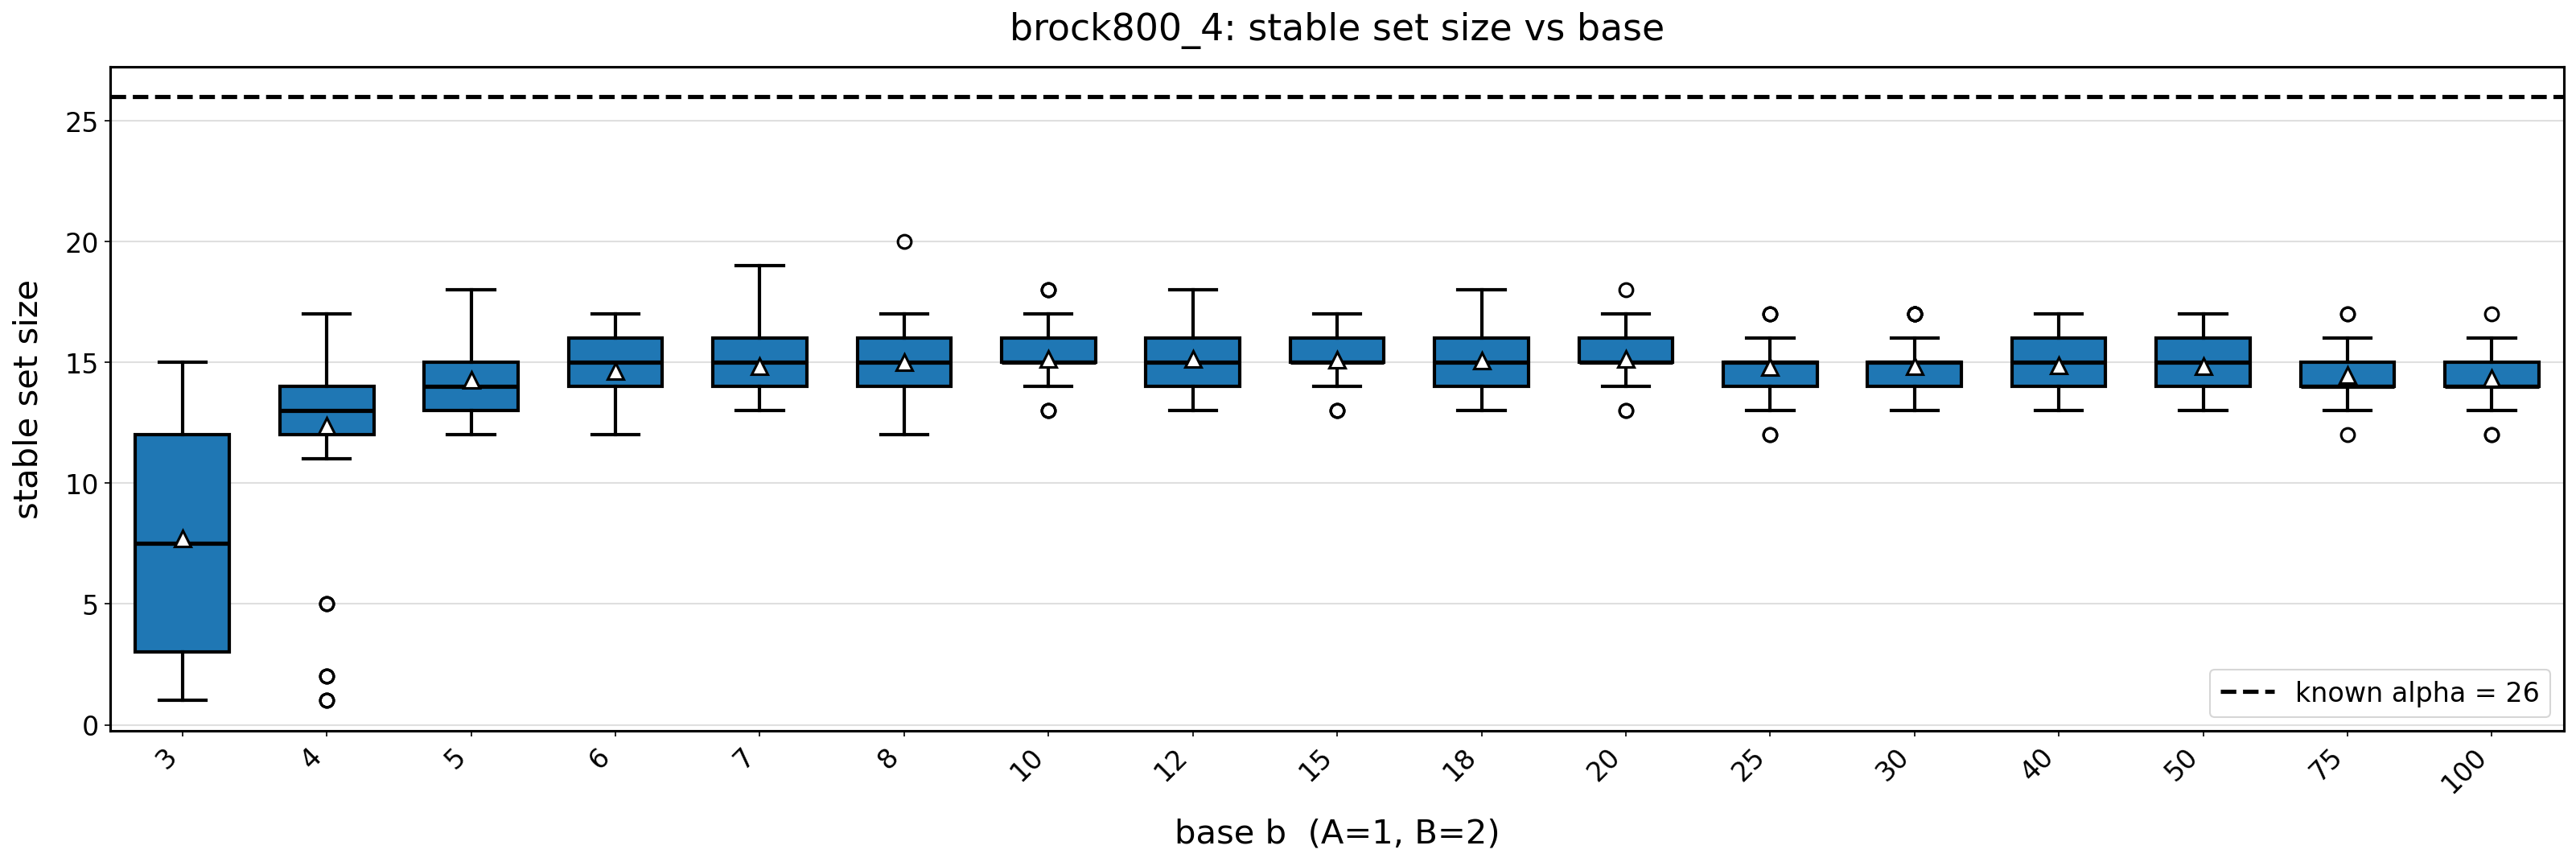
\includegraphics[width=\textwidth]{../results/boxplot_brock800_4_base.png}
            \caption{brock800\_4}
        \end{subfigure}
        \begin{subfigure}{0.75\textwidth}
            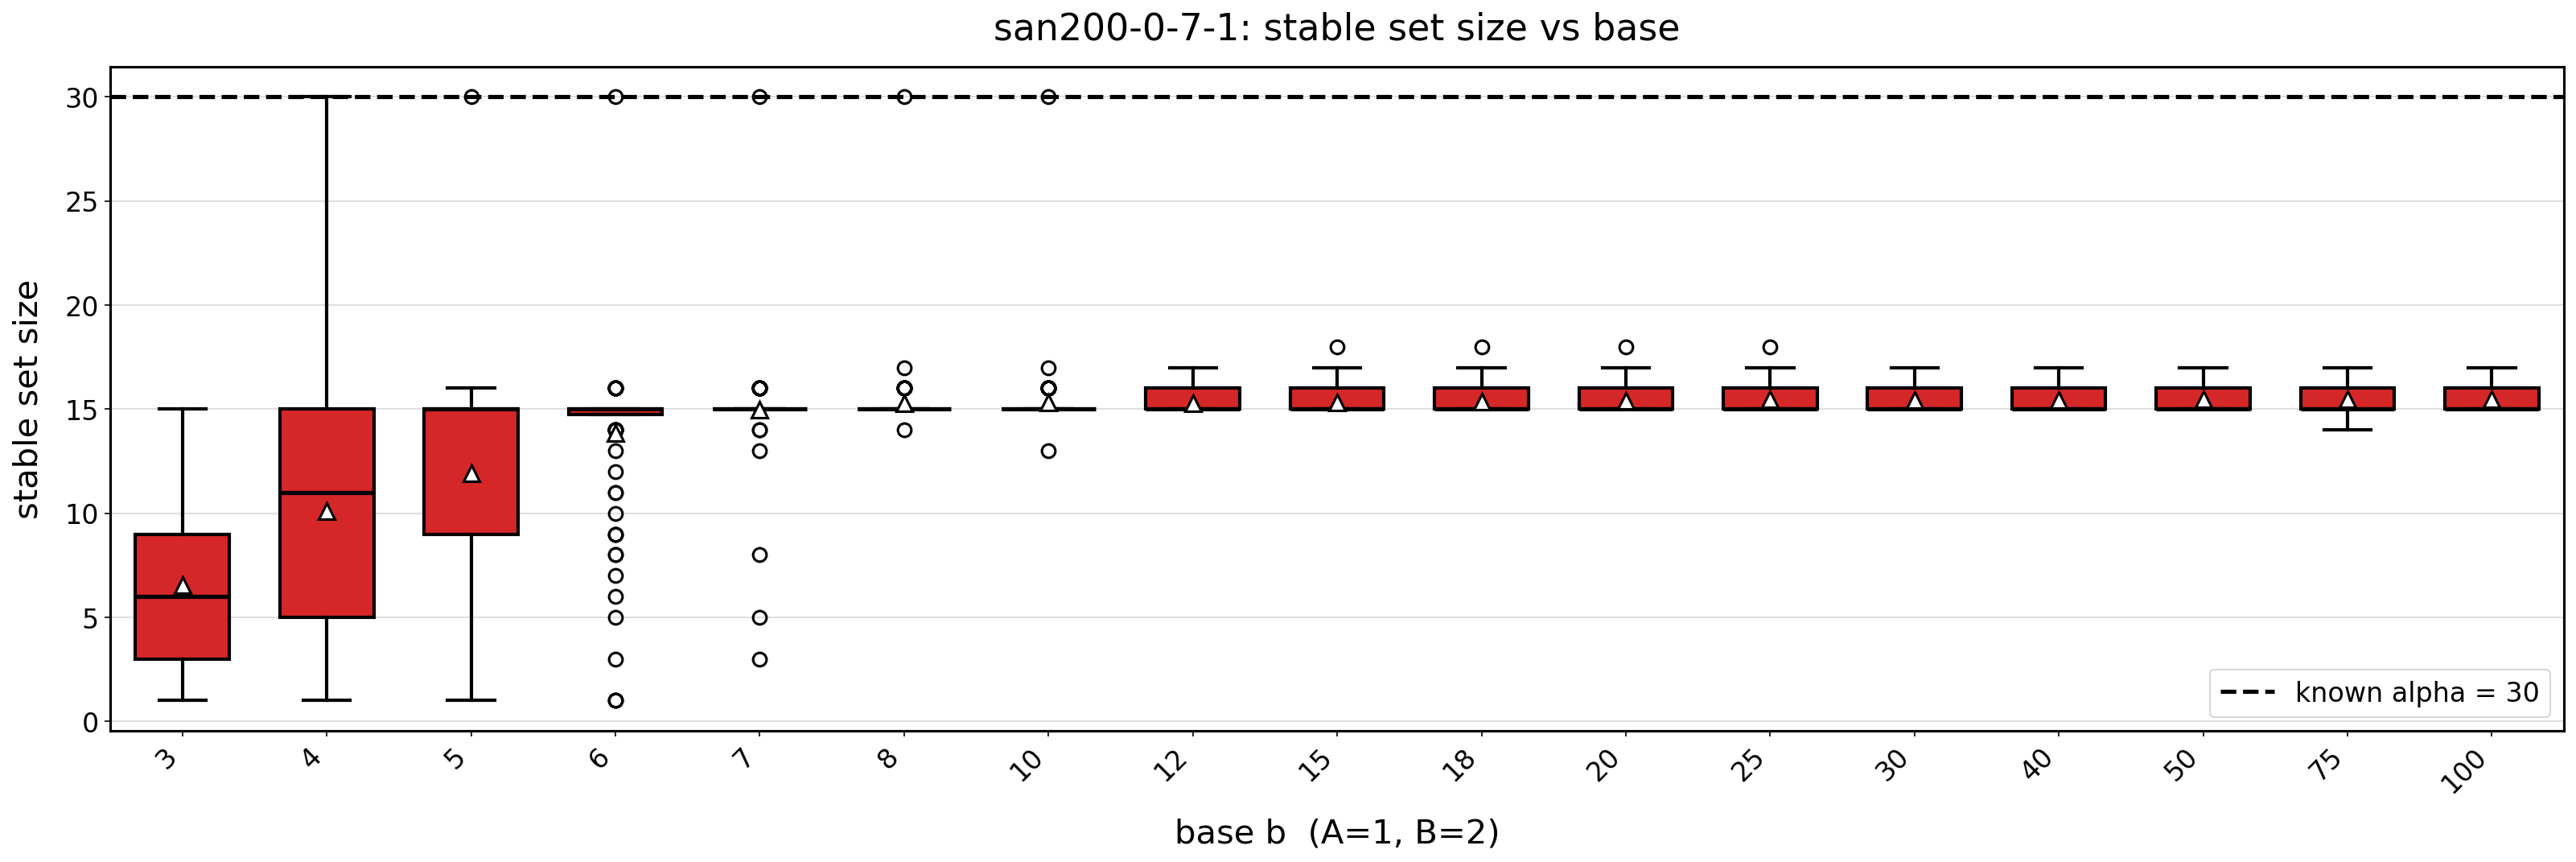
\includegraphics[width=\textwidth]{../results/boxplot_san200-0-7-1_base.png}
            \caption{san200-0-7-1}
        \end{subfigure}
        \begin{subfigure}{0.75\textwidth}
            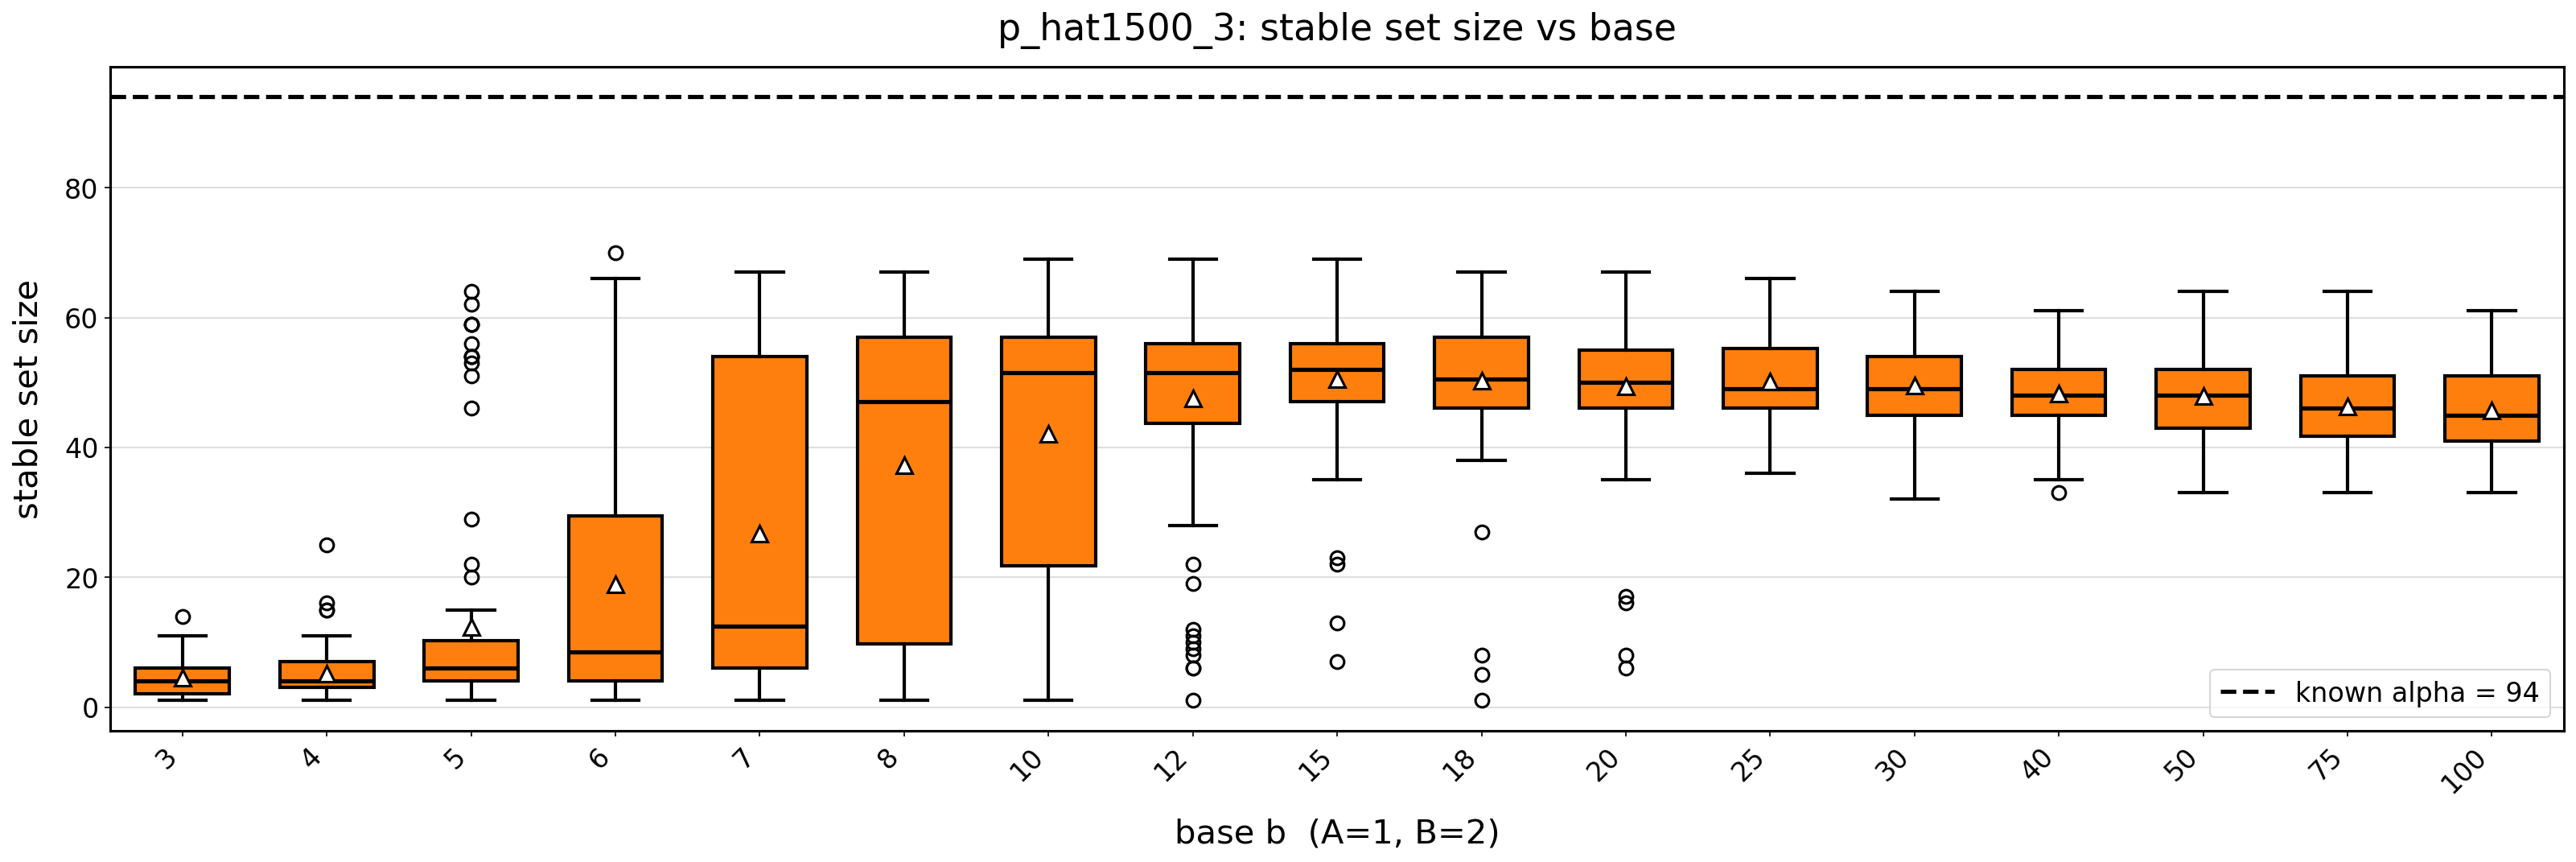
\includegraphics[width=\textwidth]{../results/boxplot_p_hat1500_3_base.png}
            \caption{p\_hat1500\_3}
        \end{subfigure}
        \begin{subfigure}{0.75\textwidth}
            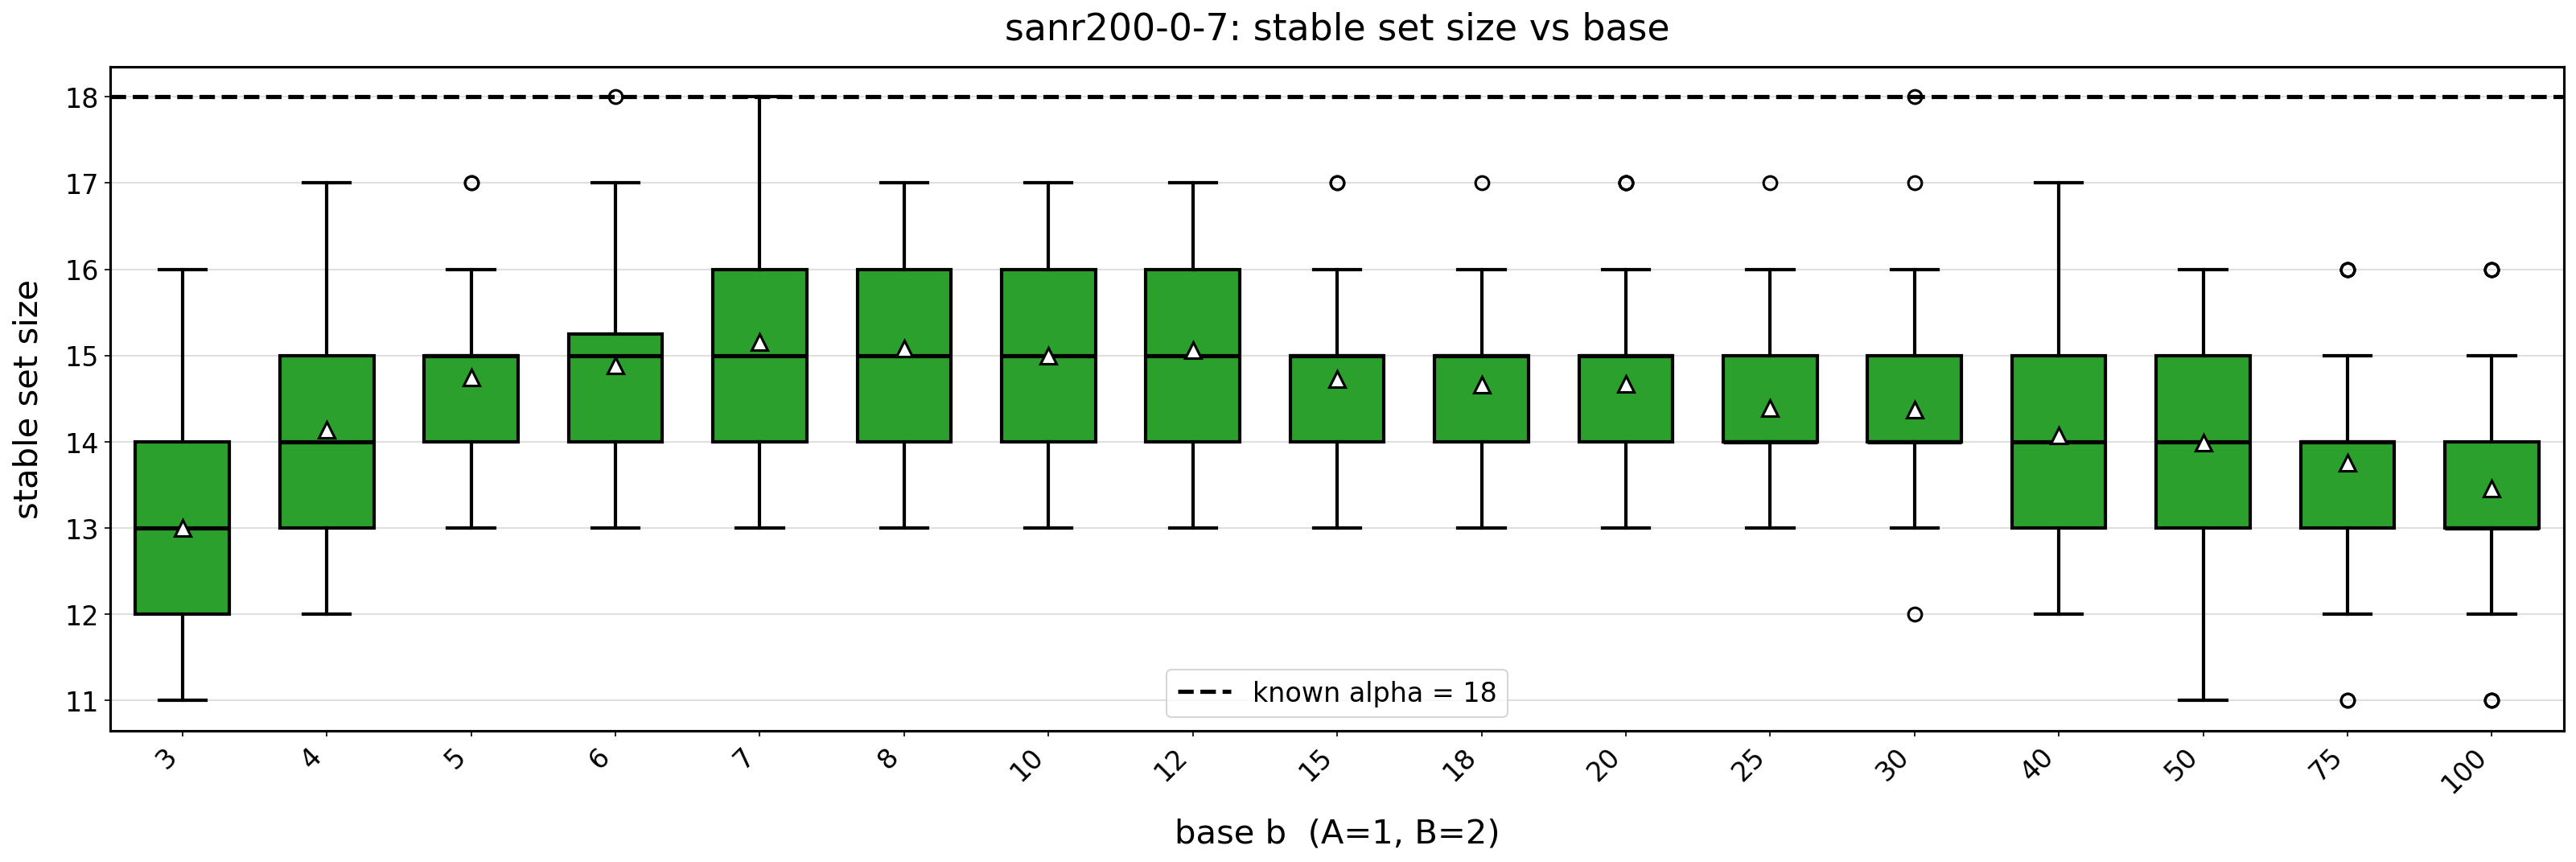
\includegraphics[width=\textwidth]{../results/boxplot_sanr200-0-7_base.png}
            \caption{sanr200-0-7}
            \label{fig:results_sanr200-0-7}
        \end{subfigure}
        \caption{Rezultati v odvisnosti od baze $b$ pri fiksnih vrednostih $A = 1.0$ in $B = 2.0$.}
        \label{fig:results_base}
    \end{figure}
    \begin{figure}[H]
        \centering
        \begin{subfigure}{0.45\textwidth}
            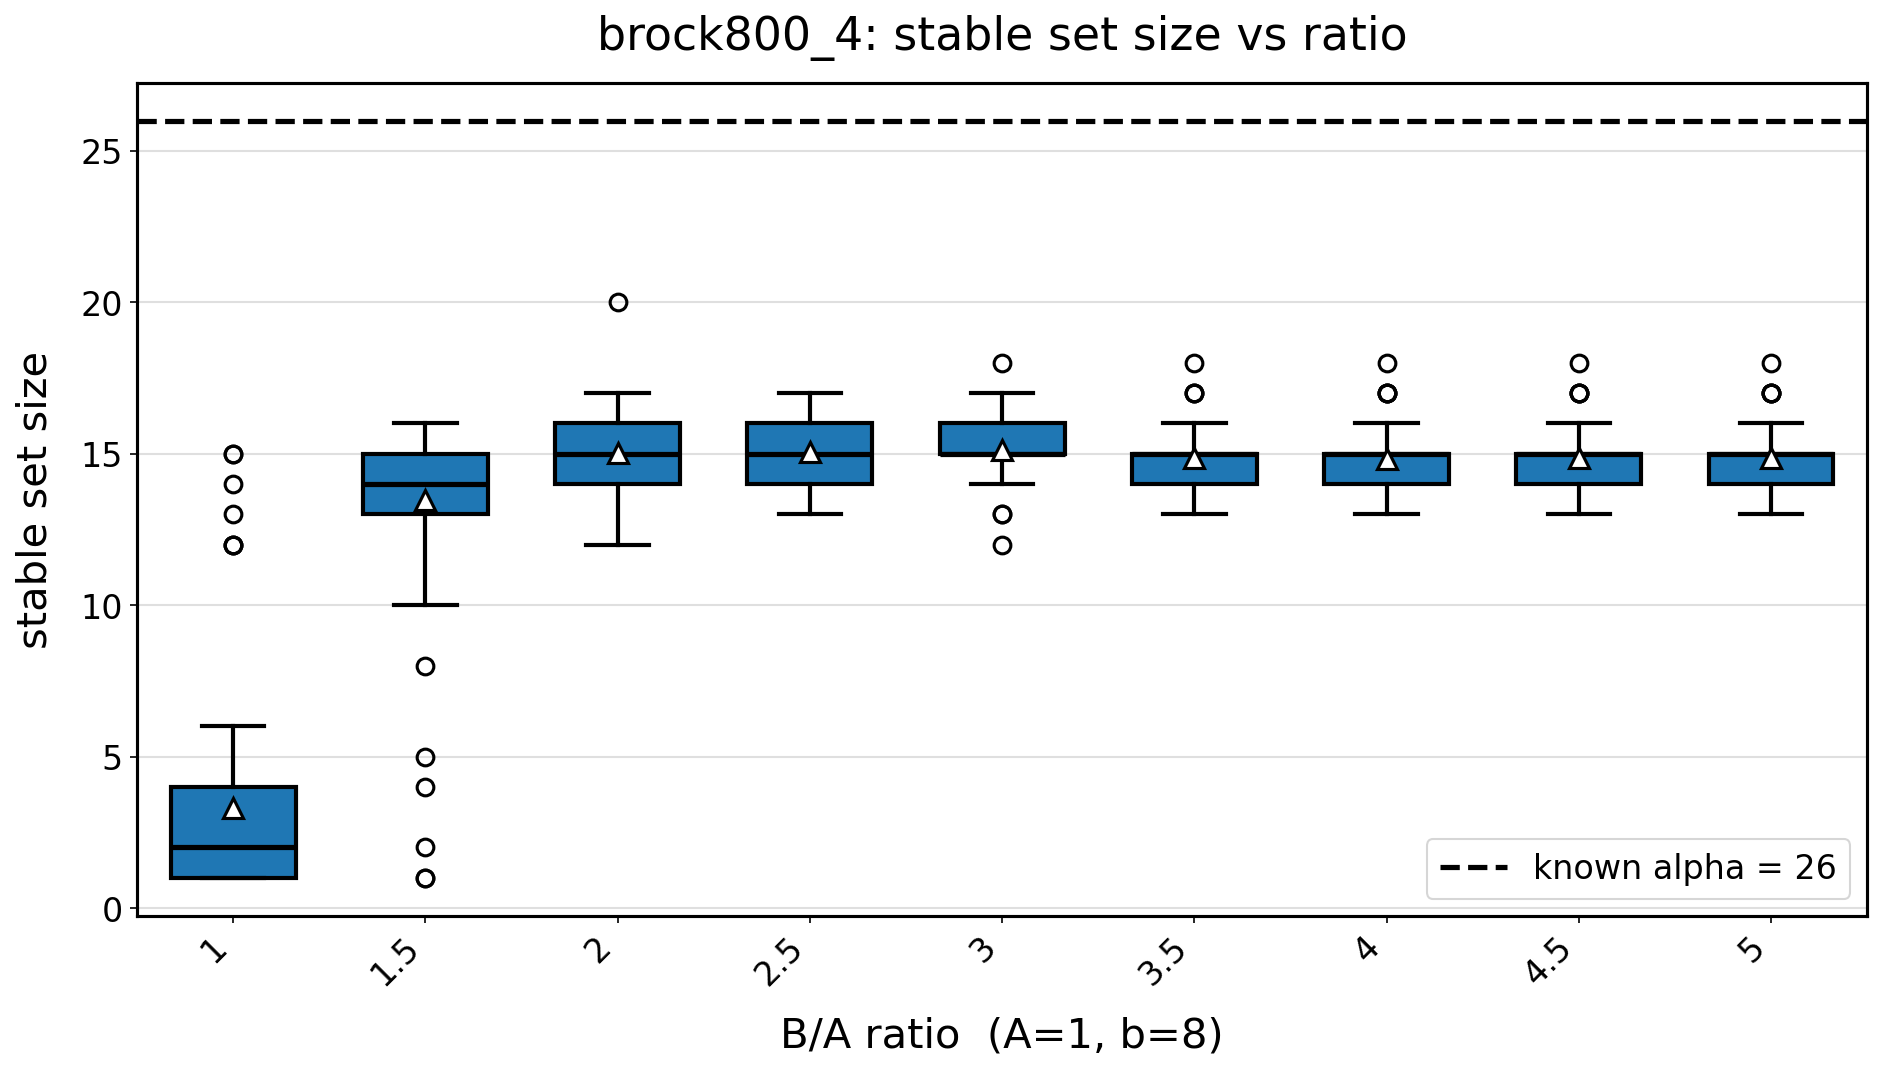
\includegraphics[width=\textwidth]{../results/boxplot_brock800_4_ratio.png}
            \caption{brock800\_4}
        \end{subfigure}
        \begin{subfigure}{0.45\textwidth}
            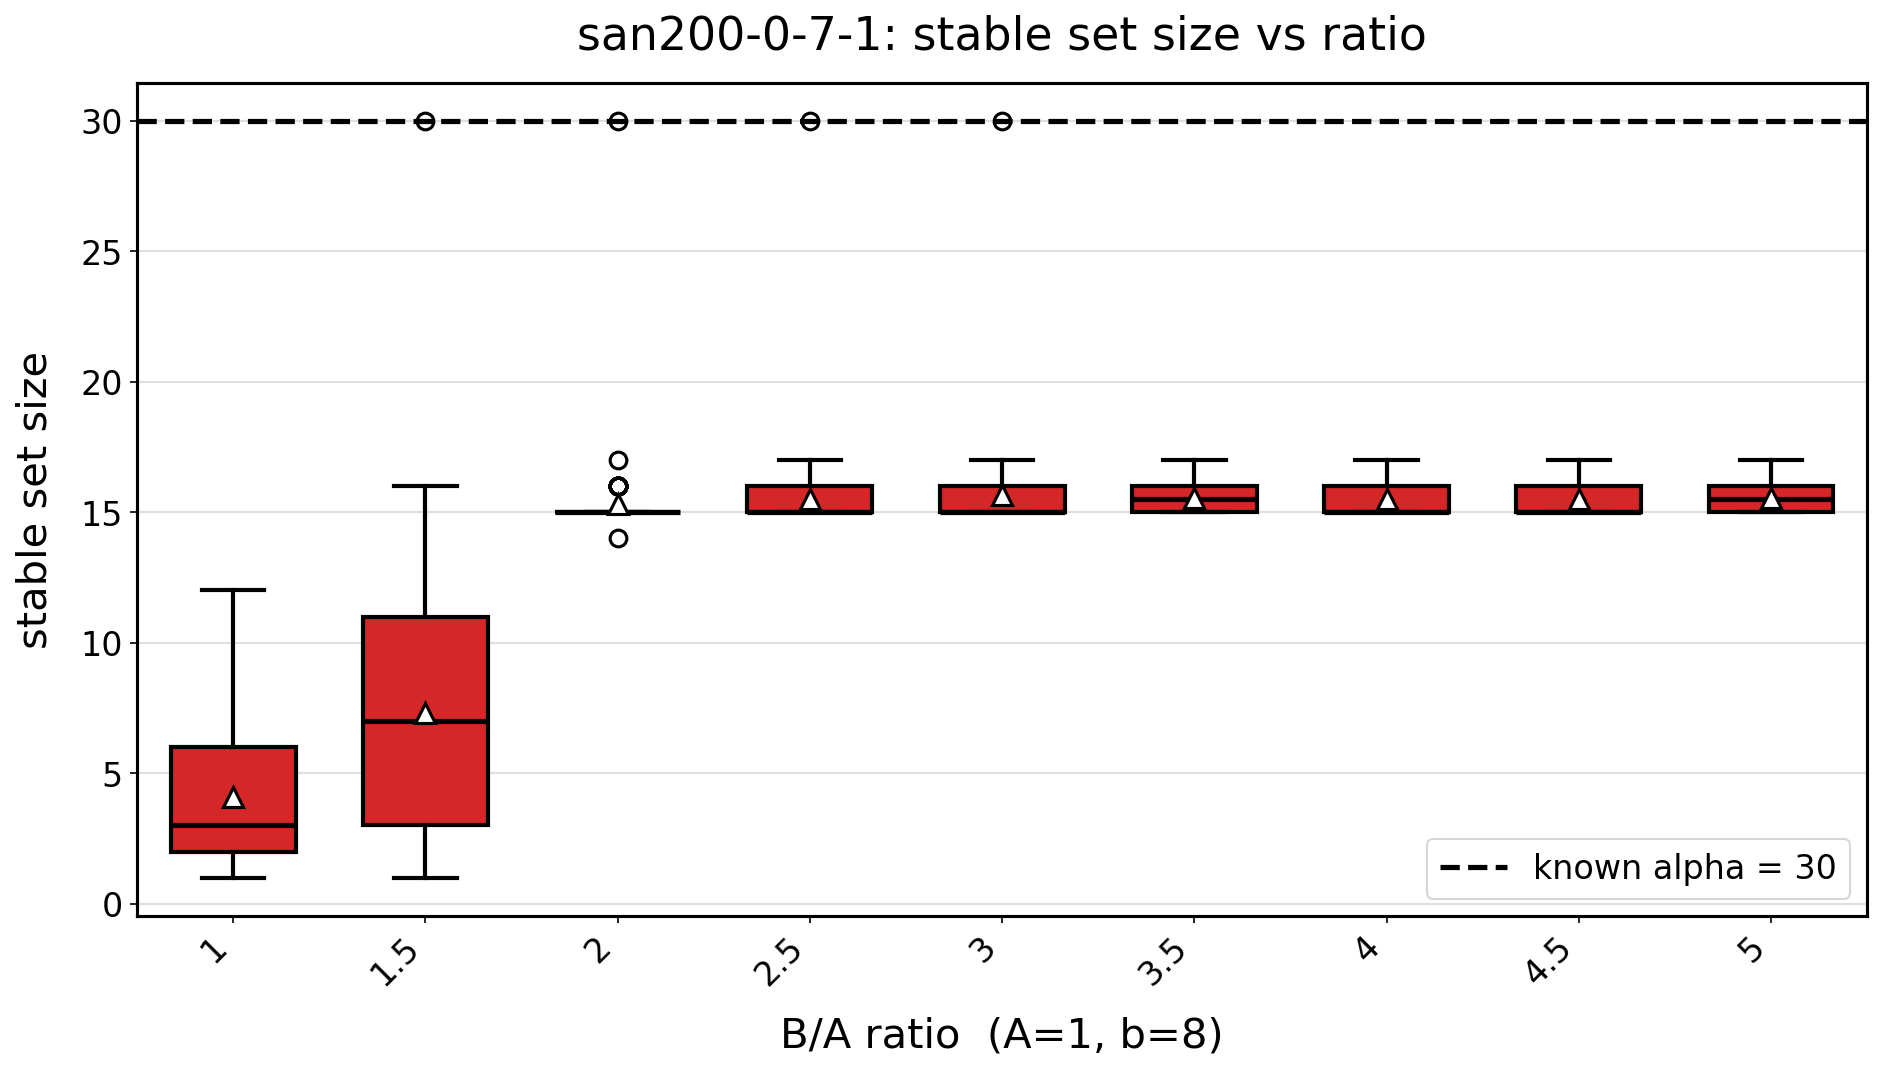
\includegraphics[width=\textwidth]{../results/boxplot_san200-0-7-1_ratio.png}
            \caption{san200-0-7-1}
        \end{subfigure}
        \begin{subfigure}{0.45\textwidth}
            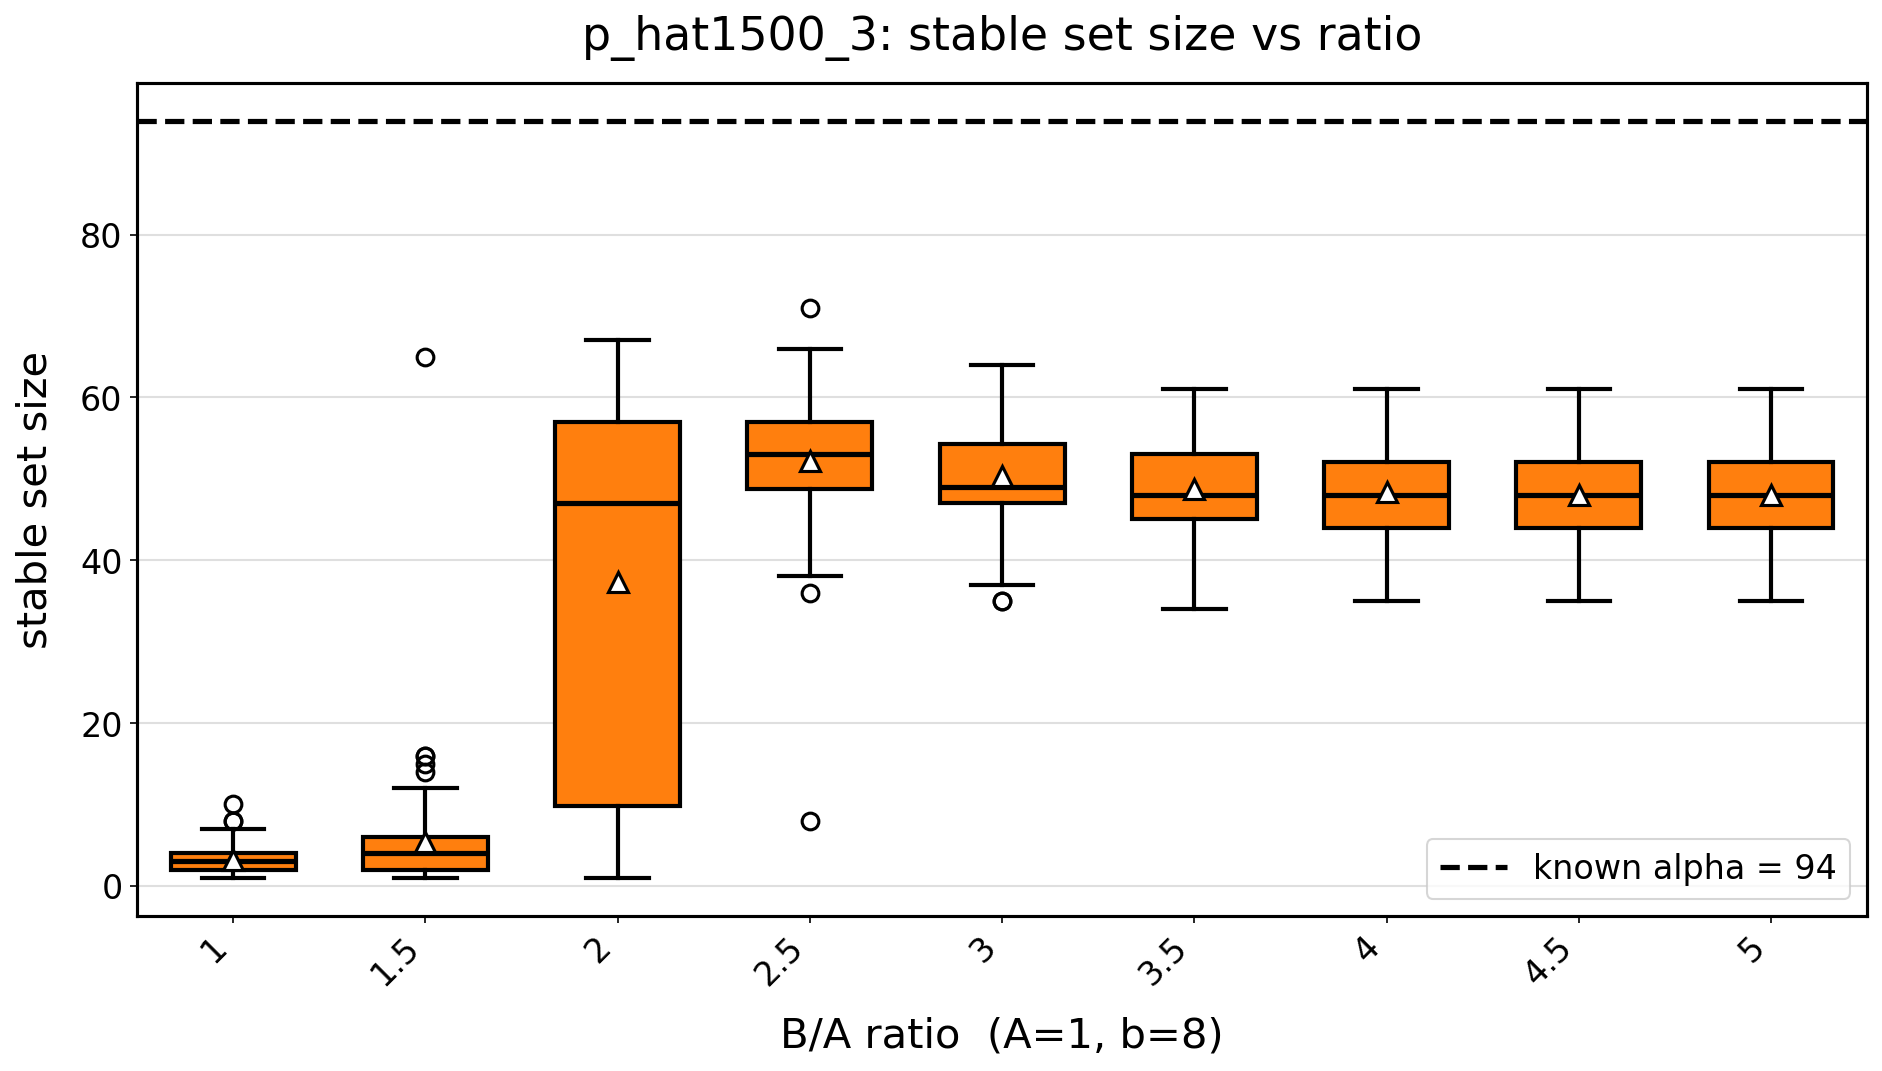
\includegraphics[width=\textwidth]{../results/boxplot_p_hat1500_3_ratio.png}
            \caption{p\_hat1500\_3}
        \end{subfigure}
        \begin{subfigure}{0.45\textwidth}
            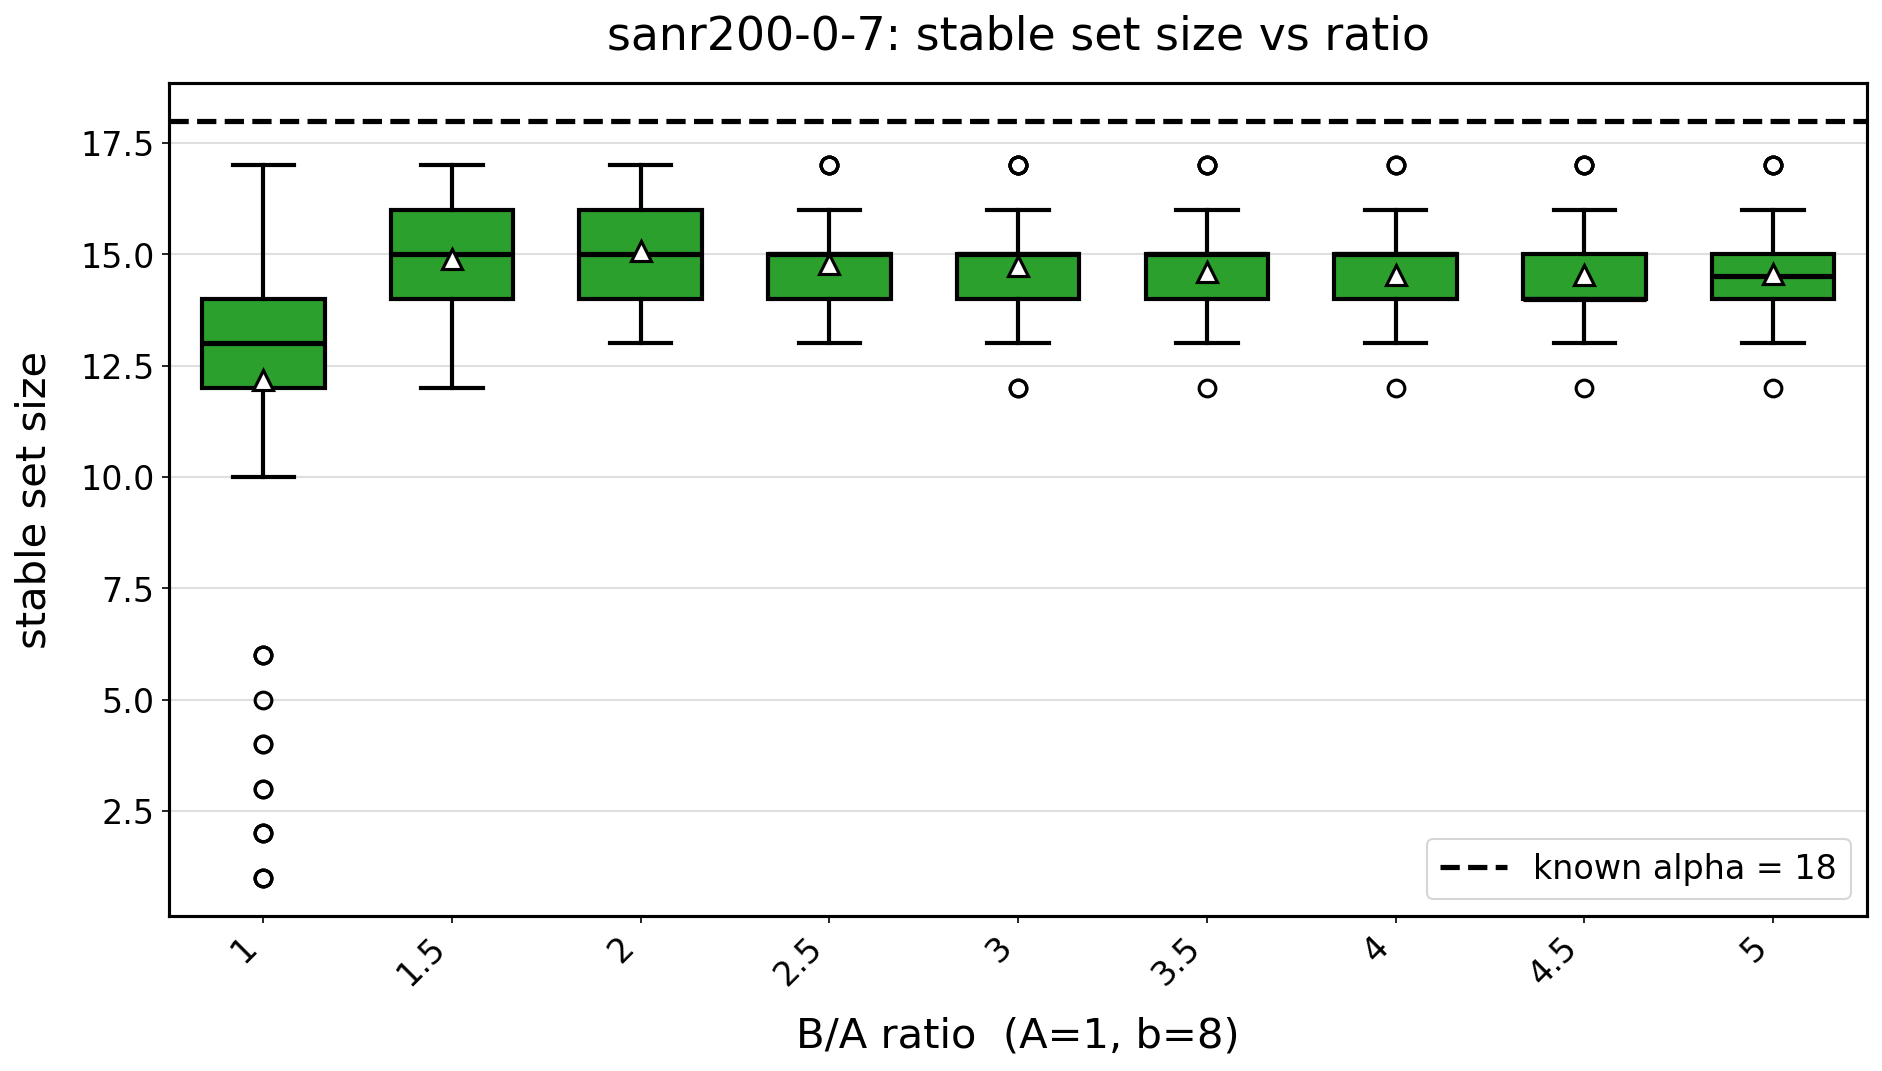
\includegraphics[width=\textwidth]{../results/boxplot_sanr200-0-7_ratio.png}
            \caption{sanr200-0-7-1}
        \end{subfigure}
        \caption{Rezultati v odvisnosti od razmerja $B/A$ pri fiksni vrednosti baze $b = 4$.}
        \label{fig:results_ratio}
    \end{figure}
    \begin{figure}[H]
        \centering
        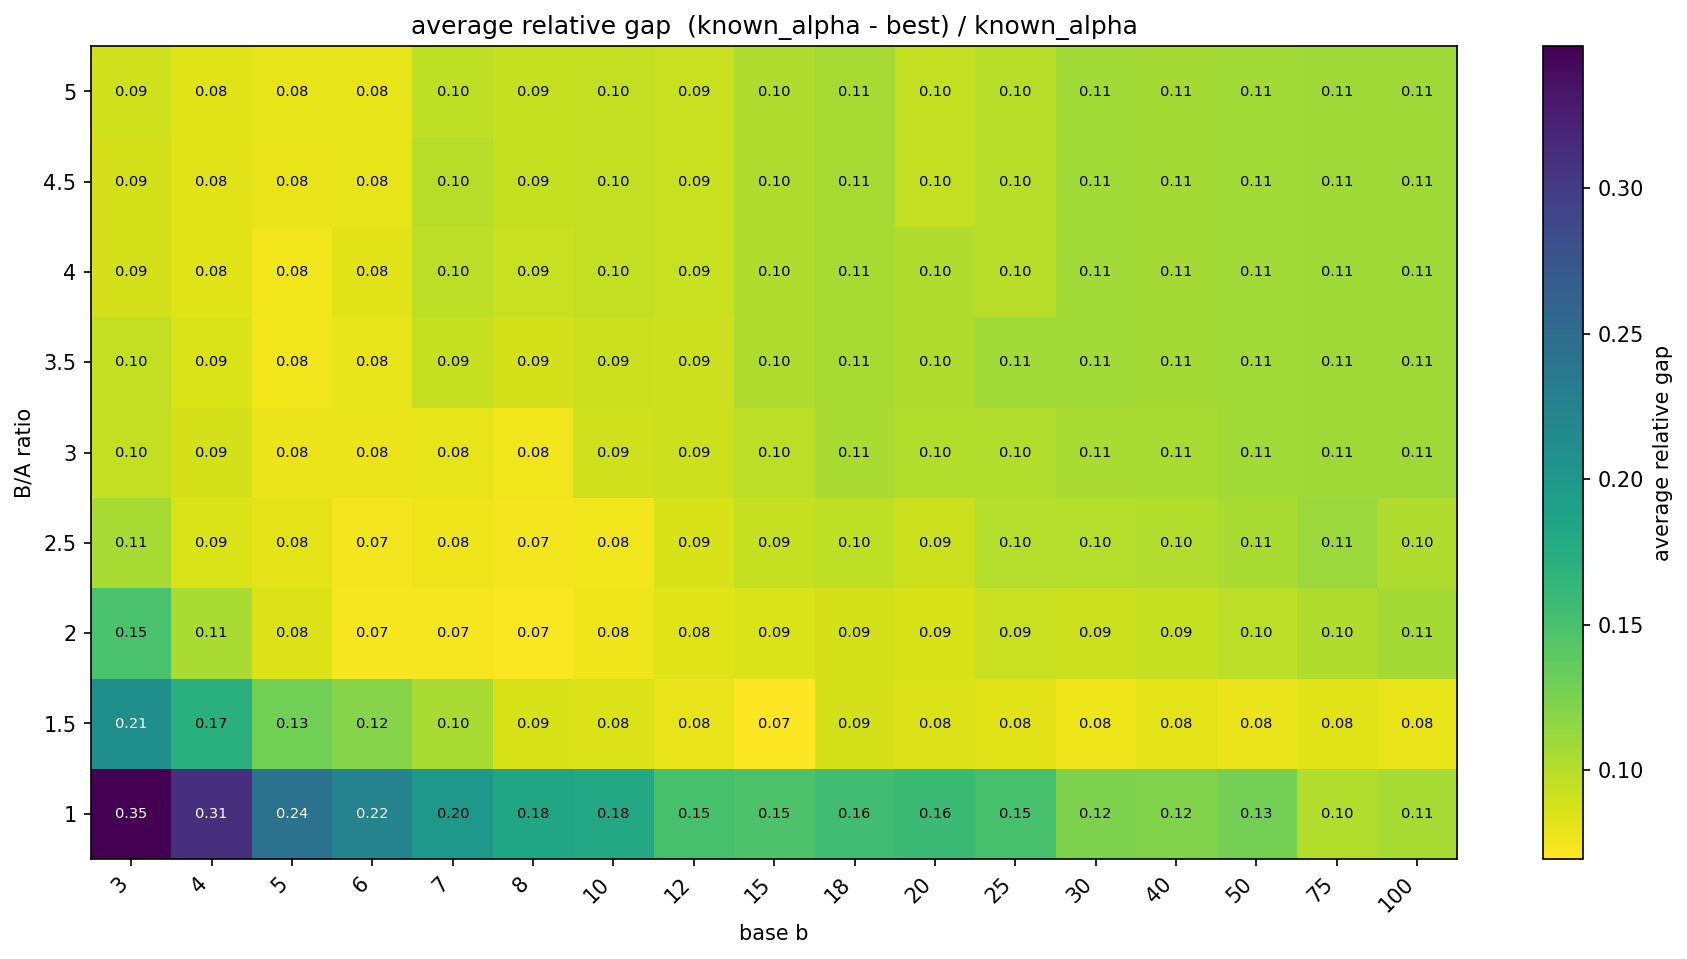
\includegraphics[width=0.8\textwidth]{../results/param_sweep_gap_heatmap.png}
        \caption{Rezultati v odvisnosti od baze $b$ in razmerja $B/A$.}
        \label{fig:results_heatmap}
    \end{figure}
    Nato sem s temi parametri izvedel algoritem na vseh instancah iz DIMACS seta, rezultati pa so prikazani v tabeli \ref{tab:results}.
    Takšen algoritem, brez kakršnihkoli prilagoditev najde optimalno rešitev za $30$ od $38$ instanc.
    Stolpci si sledijo po naslednjem vrstnem redu: ime instance, število vozlišč, število povezav, število iteracij, število ponovitev, najboljša najdena stabilna množica, povprečna velikost stabilne množice, čas izvajanja v sekundah, najboljša znana stabilna množica, razlika med najboljšo najdeno in najboljšo znano stabilno množico.
    \begin{table}[H]
        \centering
        \resizebox{\columnwidth}{!}{%
        \begin{tabular}{lrrrrrrrrr}
\toprule
instance & n & m & max\_iters & num\_attempts & best & mean & time\_sec & known\_alpha & gap \\
\midrule
C125.9 & 125 & 787 & 1000000 & 100 & 34 & 34.00 & 2.76 & 34 & 0 \\
MANN\_a9 & 45 & 72 & 1000000 & 100 & 16 & 16.00 & 2.80 & 16 & 0 \\
brock200-4 & 200 & 6811 & 1000000 & 100 & 17 & 15.95 & 1.94 & 17 & 0 \\
brock800\_1 & 800 & 112095 & 1000000 & 100 & 20 & 18.32 & 2.15 & 23 & 3 \\
brock800\_2 & 800 & 111434 & 1000000 & 100 & 20 & 18.48 & 1.97 & 24 & 4 \\
brock800\_3 & 800 & 112267 & 1000000 & 100 & 19 & 18.33 & 1.94 & 25 & 6 \\
brock800\_4 & 800 & 111957 & 1000000 & 100 & 20 & 18.45 & 1.94 & 26 & 6 \\
c-fat200-1 & 200 & 18366 & 1000000 & 100 & 12 & 11.07 & 2.02 & 12 & 0 \\
c-fat200-2 & 200 & 16665 & 1000000 & 100 & 24 & 22.25 & 2.35 & 24 & 0 \\
c-fat200-5 & 200 & 11427 & 1000000 & 100 & 58 & 57.17 & 3.18 & 58 & 0 \\
c-fat500-1 & 500 & 120291 & 1000000 & 100 & 14 & 12.59 & 1.97 & 14 & 0 \\
c-fat500-2 & 500 & 115611 & 1000000 & 100 & 26 & 25.12 & 2.37 & 26 & 0 \\
c-fat500-5 & 500 & 101559 & 1000000 & 100 & 64 & 62.54 & 3.31 & 64 & 0 \\
dsjc125.5 & 125 & 3859 & 1000000 & 100 & 10 & 10.00 & 1.94 & 10 & 0 \\
dsjc125.9 & 125 & 789 & 1000000 & 100 & 34 & 33.99 & 2.40 & 34 & 0 \\
evil-N120-p98-chv12x10 & 120 & 545 & 1000000 & 100 & 20 & 20.00 & 2.52 & 20 & 0 \\
evil-N120-p98-myc5x24 & 120 & 236 & 1000000 & 100 & 48 & 48.00 & 2.87 & 48 & 0 \\
evil-N121-p98-myc11x11 & 121 & 508 & 1000000 & 100 & 22 & 22.00 & 2.47 & 22 & 0 \\
evil-N125-p98-s3m25x5 & 125 & 873 & 1000000 & 100 & 20 & 20.00 & 2.24 & 20 & 0 \\
hamming6\_2 & 64 & 192 & 1000000 & 100 & 32 & 32.00 & 3.61 & 32 & 0 \\
hamming6\_4 & 64 & 1312 & 1000000 & 100 & 4 & 4.00 & 2.40 & 4 & 0 \\
johnson16\_2\_4 & 120 & 1680 & 1000000 & 100 & 8 & 8.00 & 2.52 & 8 & 0 \\
johnson8\_2\_4 & 28 & 168 & 1000000 & 100 & 4 & 4.00 & 2.77 & 4 & 0 \\
johnson8\_4\_4 & 70 & 560 & 1000000 & 100 & 14 & 14.00 & 2.73 & 14 & 0 \\
keller4 & 171 & 5100 & 1000000 & 100 & 11 & 11.00 & 2.54 & 11 & 0 \\
p-hat500-1 & 500 & 93181 & 1000000 & 100 & 9 & 8.99 & 2.37 & 9 & 0 \\
p\_hat1500\_1 & 1500 & 839327 & 1000000 & 100 & 11 & 10.16 & 2.55 & 12 & 1 \\
p\_hat1500\_2 & 1500 & 555290 & 1000000 & 100 & 64 & 61.79 & 2.97 & 65 & 1 \\
p\_hat1500\_3 & 1500 & 277006 & 1000000 & 100 & 91 & 87.62 & 2.83 & 94 & 3 \\
paley101 & 101 & 2525 & 1000000 & 100 & 5 & 5.00 & 2.56 & 5 & 0 \\
paley61 & 61 & 915 & 1000000 & 100 & 5 & 5.00 & 2.59 & 5 & 0 \\
paley73 & 73 & 1314 & 1000000 & 100 & 5 & 5.00 & 2.49 & 5 & 0 \\
paley89 & 89 & 1958 & 1000000 & 100 & 5 & 5.00 & 2.48 & 5 & 0 \\
paley97 & 97 & 2328 & 1000000 & 100 & 6 & 6.00 & 2.43 & 6 & 0 \\
san200-0-7-1 & 200 & 5970 & 1000000 & 100 & 30 & 15.77 & 3.48 & 30 & 0 \\
san200-0-7-2 & 200 & 5970 & 1000000 & 100 & 14 & 12.81 & 3.57 & 18 & 4 \\
sanr200-0-7 & 200 & 6032 & 1000000 & 100 & 18 & 17.95 & 2.50 & 18 & 0 \\
\bottomrule
\end{tabular}

        }
        \caption{Rezultati izvajanja algoritma na testnih instancah. Za vse primere so bili uporabljeni parametri $A = 1.0$, $B = 2.0$, baza $b = 8$. Število ponovitev in število iteracij pa sta bili konstantni.}
        \label{tab:results}
    \end{table}

    \subsection{Čas izvajanja in optimalnost rezultatov}
    Število iteracij in ponovitev v prejšnji tabeli je bilo izbrano precej arbitrarno.
    Ker je to glavni faktor kako dobro rešitev bo algoritem našel bom v nadaljevanju preveril vpliv tega.
    Slika \ref{fig:results_time_to_best_vs_gap} prikazuje optimalnost rešitve v odvisnosti od časa izvajanja ene ponovitve algoritma, barva pa prikazuje število iteracij.
    Izbral sem nekaj različnih vrednosti parametra $max\_iters$ in za vsako izvedel $20$ ponovitev algoritma, rezultati za vsako število iteracij so prikazani z boxplotom.\\
    \begin{figure}[H]
        \centering
        \begin{subfigure}{0.45\textwidth}
            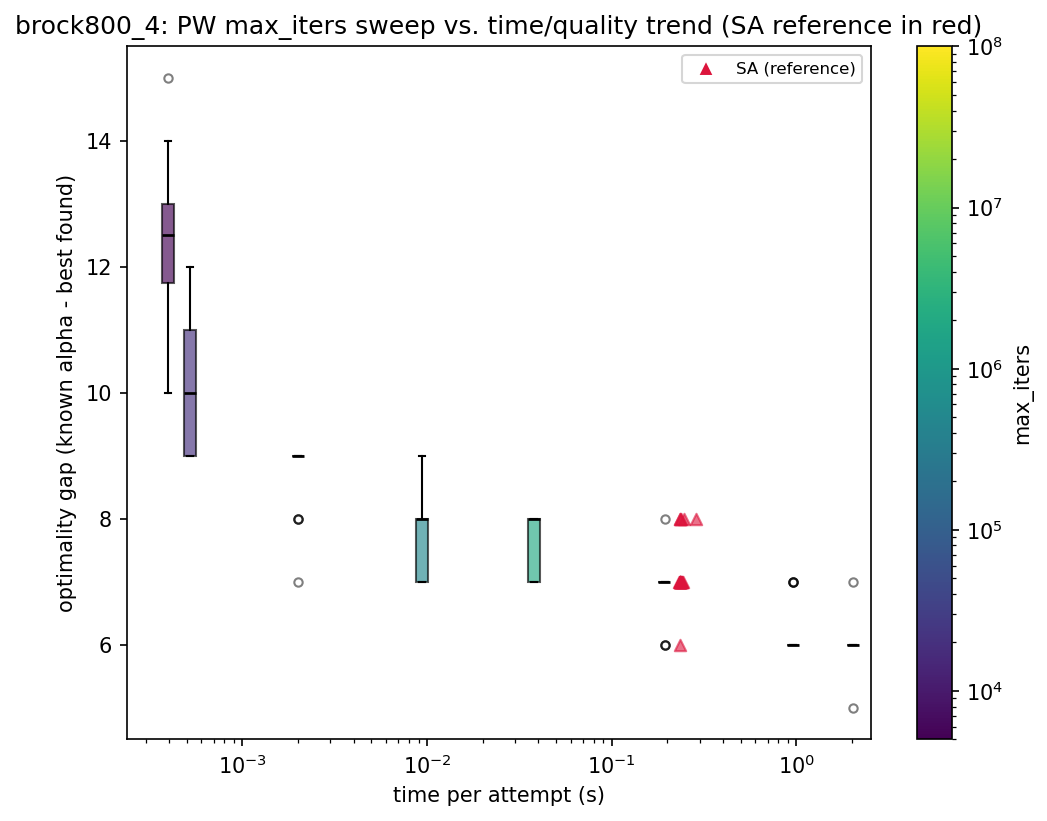
\includegraphics[width=\textwidth]{../results/time_to_best_vs_gap_brock800_4_maxiters_sweep.png}
            \caption{brock800\_4}
        \end{subfigure}
        \begin{subfigure}{0.45\textwidth}
            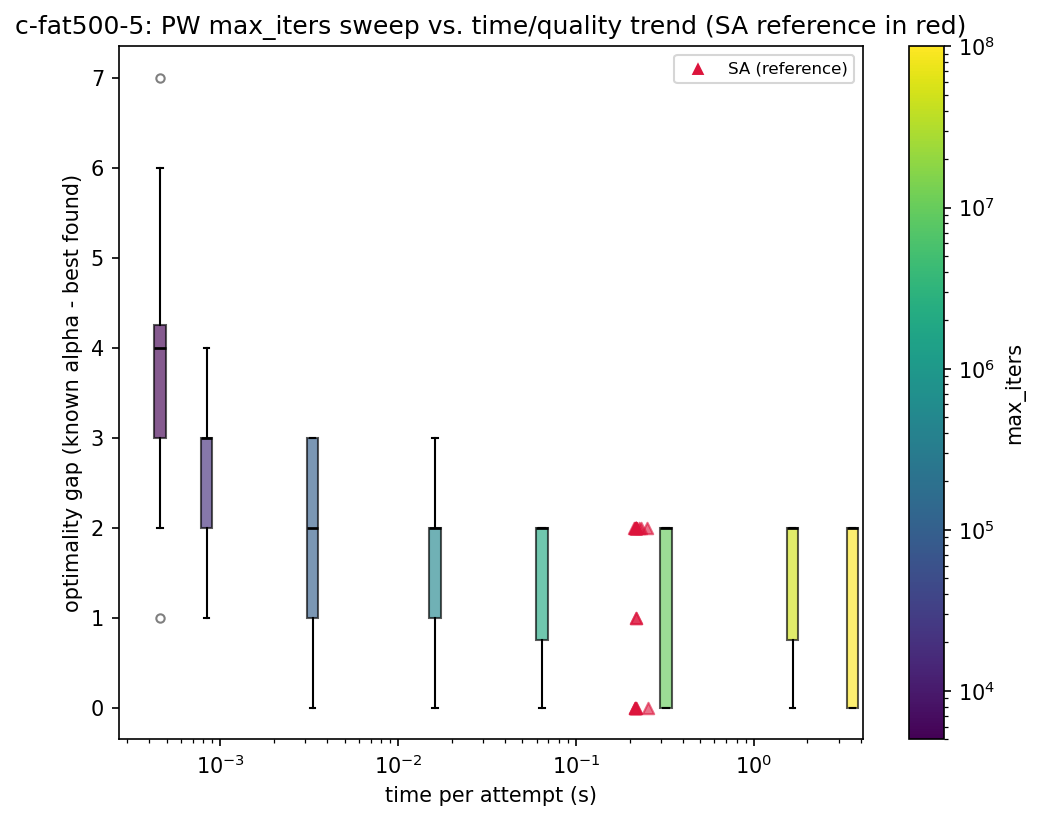
\includegraphics[width=\textwidth]{../results/time_to_best_vs_gap_c-fat500-5_maxiters_sweep.png}
            \caption{c-fat500-5}
        \end{subfigure}
        \begin{subfigure}{0.45\textwidth}
            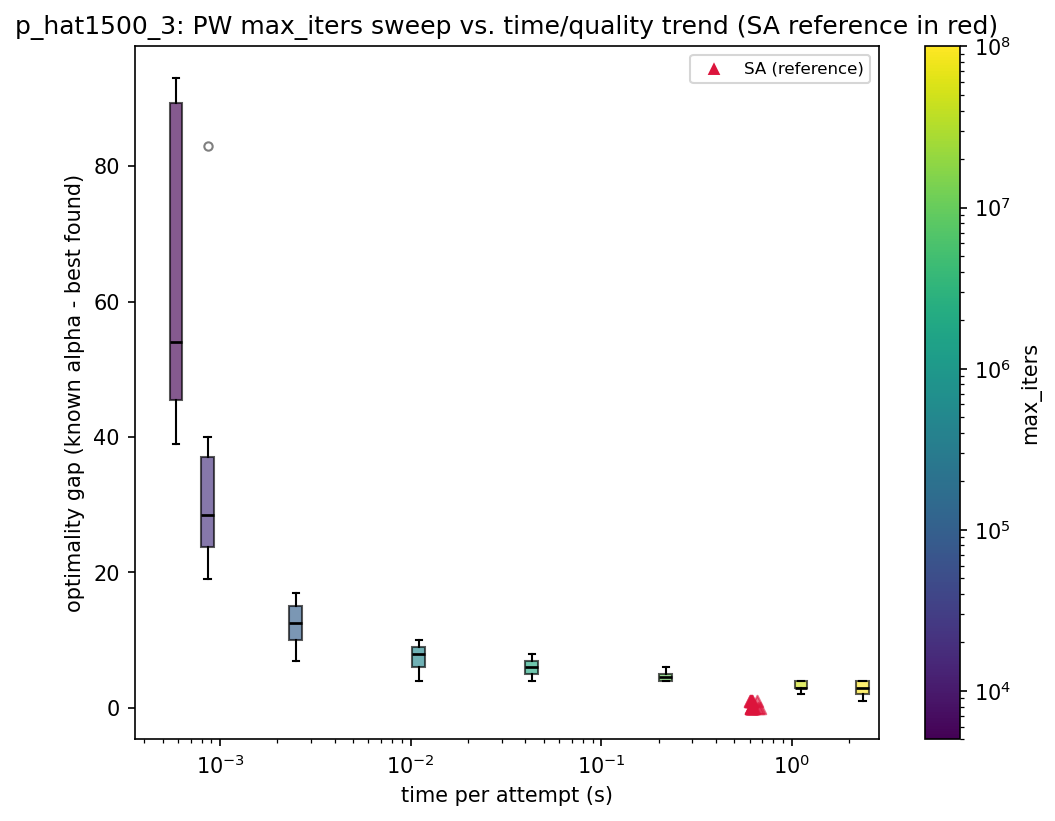
\includegraphics[width=\textwidth]{../results/time_to_best_vs_gap_p_hat1500_3_maxiters_sweep.png}
            \caption{p\_hat1500\_3}
        \end{subfigure}
        \begin{subfigure}{0.45\textwidth}
            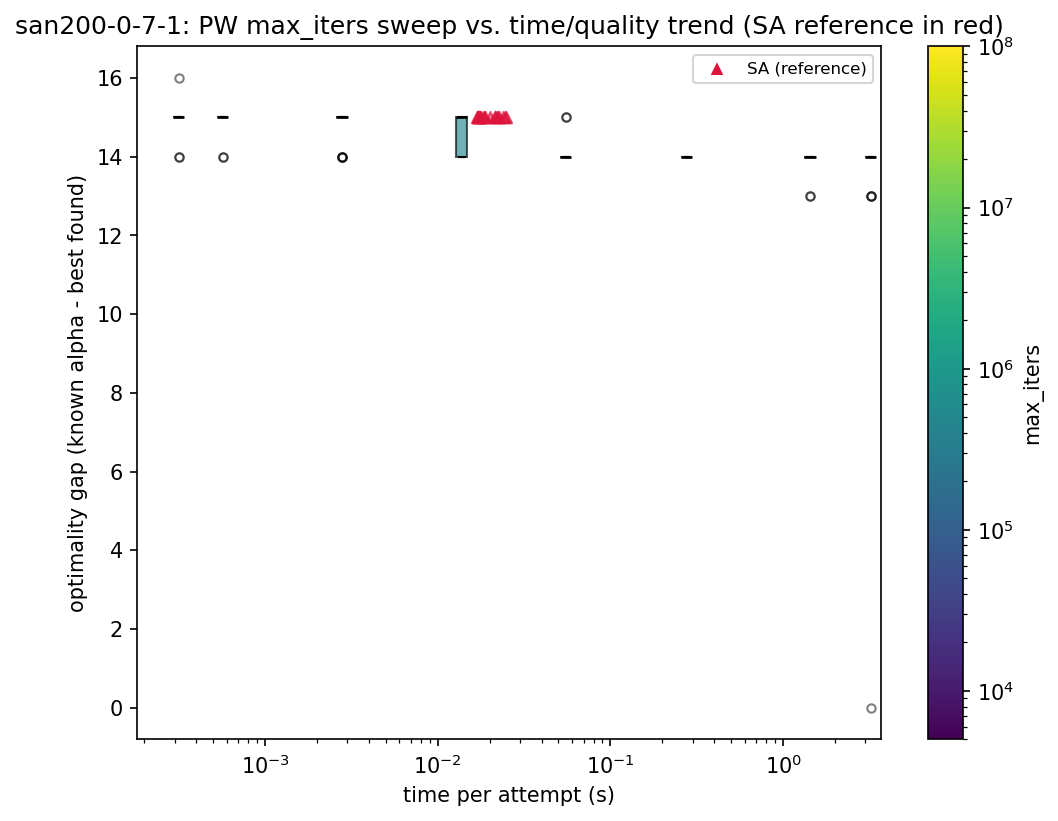
\includegraphics[width=\textwidth]{../results/time_to_best_vs_gap_san200-0-7-1_maxiters_sweep.png}
            \caption{san200-0-7-1}
        \end{subfigure}
        \caption{Optimalnost rešitve v odvisnosti od časa izvajanja ene ponovitve algoritma, barva pa prikazuje število iteracij.}
        \label{fig:results_time_to_best_vs_gap}
    \end{figure}

    \subsection{Začetek na greedy rešitvi}
    Algoritem zmeraj začne z prazno stabilno množico in potem postopoma dodaja vozlišča.
    Hitrost bi lahko izboljšali, če začnemo z že obstoječo stabilno množico, ki je morda blizu optimalne rešitve.
    Zato sem dodal možnost, da algoritem najprej izvede greedy algoritem, ki najde neko stabilno množico in potem začne z algoritmom.
    Začnemo torej z prazno množico in najprej naključno dodajamo vozlišča, ki niso povezana s povezavo z že izbrano množico, dokler ne pridemo do neke stabilne množice, ki jo potem uporabimo kot začetno stanje algoritma.
    Primerjavo med začetkom z greedy rešitvijo in začetkom z prazno množico prikazuje spodnja slika \ref{fig:greedy_start_compare}, kjer je prikazana enaka stvar, kot na prejšnjih slikah, le da je sedaj z barvo označen način začetka algoritma.
    Modra barva označuje začetek z prazno množico, oranžna pa označuje začetek z greedy rešitvijo.
    Vidimo, da takšen postopek ne izboljša najdene rešitve, edina razlika je, da začetni korak traja dlje časa, zato so rešitve za majhen čas izvajanja slabše, kot če bi začeli z prazno množico.
    Tu je največji faktor to, da je koda za inicializacijo slabše optimizirana.
    \begin{figure}[H]
        \centering
        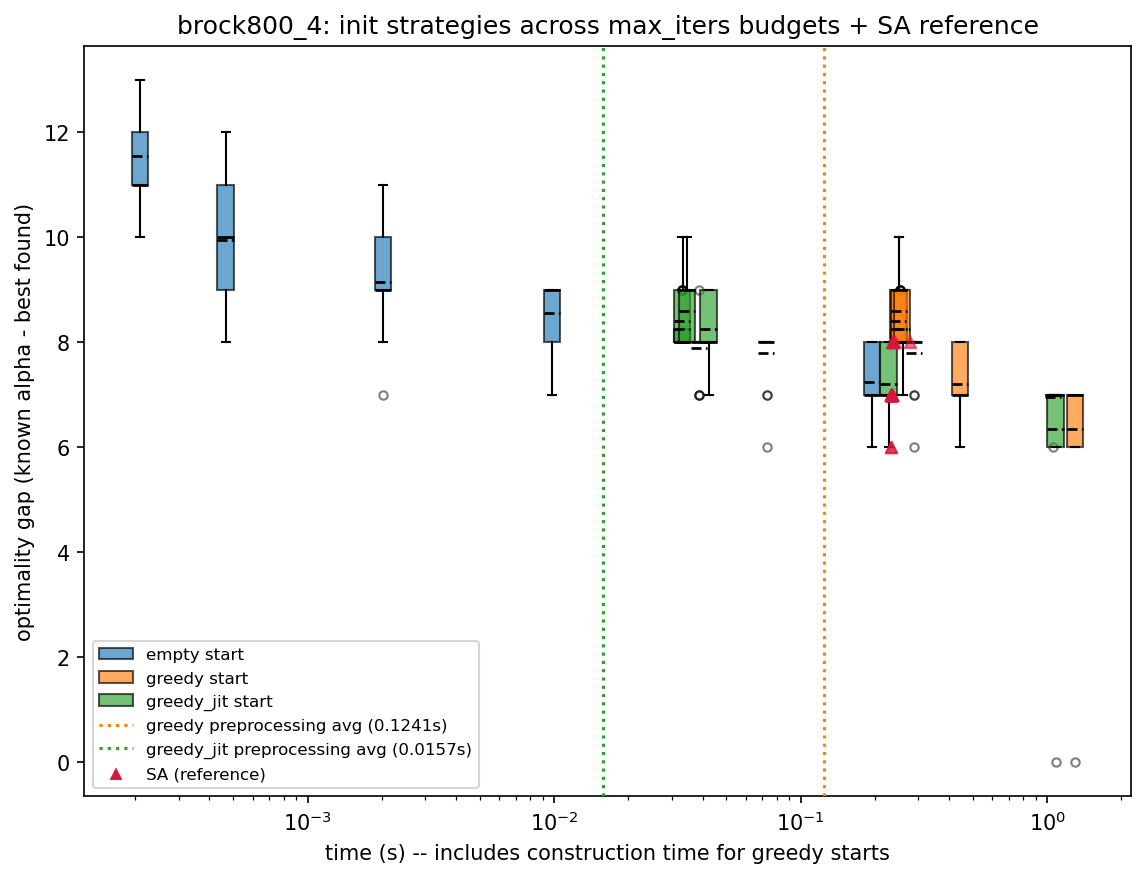
\includegraphics[width=0.5\textwidth]{../results/greedy_start_compare_brock800_4.png}
        \caption{Optimalnost rešitve v odvisnosti od časa izvajanja ene ponovitve algoritma, barva pa prikazuje način začetka algoritma.}
        \label{fig:greedy_start_compare}
    \end{figure}
    
    \subsection{Primerjava najboljšega stanja z končnim}
    Algoritem si tekom poteka shranjuje najboljšo rešitev, ki jo je našel.
    Opcija, ki jo lahko dodamo, je da namesto najboljše rešitve, vzamemo končno stanje, ki ga algoritem najde.
    Ta množica ponavadi sploh ni stabilna, ampak je lahko blizu optimalne rešitve, ki jo lahko popravimo tako, da postopoma odstranjujemo vozlišča, ki so povezana s povezavo.
    Primerjavo teh dveh postopkov prikazuje spodnja tabela \ref{tab:results_last_state}, kjer lahko vidimo, da je končno stanje zmeraj slabše od najboljše najdene stabilne množice, zato bom še naprej uporabljal prvotno verzijo algoritma.
    \begin{table}[H]
        \centering
        \resizebox{\columnwidth}{!}{%
        \begin{tabular}{lrrrrrrrrrrr}
\toprule
instance & n & m & max\_iters & num\_attempts & known\_alpha & avg\_best & avg\_repaired & max\_best & max\_repaired & gap\_best & gap\_repaired \\
\midrule
C125.9 & 125 & 787 & 62500 & 50 & 34 & 25.68 & 16.98 & 28 & 23 & 6 & 11 \\
MANN\_a9 & 45 & 72 & 22500 & 50 & 16 & 15.20 & 9.70 & 16 & 14 & 0 & 2 \\
brock200-4 & 200 & 6811 & 100000 & 50 & 17 & 12.60 & 7.60 & 14 & 11 & 3 & 6 \\
brock800\_1 & 800 & 112095 & 400000 & 50 & 23 & 15.36 & 10.46 & 17 & 13 & 6 & 10 \\
brock800\_2 & 800 & 111434 & 400000 & 50 & 24 & 15.34 & 10.24 & 17 & 13 & 7 & 11 \\
brock800\_3 & 800 & 112267 & 400000 & 50 & 25 & 15.20 & 9.84 & 17 & 13 & 8 & 12 \\
brock800\_4 & 800 & 111957 & 400000 & 50 & 26 & 15.34 & 10.00 & 17 & 13 & 9 & 13 \\
c-fat200-1 & 200 & 18366 & 100000 & 50 & 12 & 11.28 & 5.06 & 12 & 9 & 0 & 3 \\
c-fat200-2 & 200 & 16665 & 100000 & 50 & 24 & 18.94 & 9.80 & 21 & 16 & 3 & 8 \\
c-fat200-5 & 200 & 11427 & 100000 & 50 & 58 & 40.94 & 25.92 & 44 & 37 & 14 & 21 \\
c-fat500-1 & 500 & 120291 & 250000 & 50 & 14 & 12.28 & 5.88 & 14 & 9 & 0 & 5 \\
c-fat500-2 & 500 & 115611 & 250000 & 50 & 26 & 21.18 & 12.10 & 24 & 17 & 2 & 9 \\
c-fat500-5 & 500 & 101559 & 250000 & 50 & 64 & 44.56 & 29.50 & 48 & 43 & 16 & 21 \\
dsjc125.5 & 125 & 3859 & 62500 & 50 & 10 & 8.50 & 4.76 & 9 & 7 & 1 & 3 \\
dsjc125.9 & 125 & 789 & 62500 & 50 & 34 & 25.70 & 16.36 & 28 & 24 & 6 & 10 \\
evil-N120-p98-chv12x10 & 120 & 545 & 60000 & 50 & 20 & 20.00 & 15.60 & 20 & 18 & 0 & 2 \\
evil-N120-p98-myc5x24 & 120 & 236 & 60000 & 50 & 48 & 37.74 & 26.42 & 41 & 34 & 7 & 14 \\
evil-N121-p98-myc11x11 & 121 & 508 & 60500 & 50 & 22 & 22.00 & 15.54 & 22 & 20 & 0 & 2 \\
evil-N125-p98-s3m25x5 & 125 & 873 & 62500 & 50 & 20 & 19.48 & 13.24 & 20 & 17 & 0 & 3 \\
hamming6\_2 & 64 & 192 & 32000 & 50 & 32 & 24.58 & 13.46 & 27 & 19 & 5 & 13 \\
hamming6\_4 & 64 & 1312 & 32000 & 50 & 4 & 4.00 & 2.74 & 4 & 4 & 0 & 0 \\
johnson16\_2\_4 & 120 & 1680 & 60000 & 50 & 8 & 8.00 & 5.90 & 8 & 7 & 0 & 1 \\
johnson8\_2\_4 & 28 & 168 & 14000 & 50 & 4 & 4.00 & 2.74 & 4 & 4 & 0 & 0 \\
johnson8\_4\_4 & 70 & 560 & 35000 & 50 & 14 & 11.94 & 6.24 & 14 & 11 & 0 & 3 \\
keller4 & 171 & 5100 & 85500 & 50 & 11 & 9.74 & 5.96 & 11 & 9 & 0 & 2 \\
p-hat500-1 & 500 & 93181 & 250000 & 50 & 9 & 7.98 & 4.34 & 9 & 7 & 0 & 2 \\
p\_hat1500\_1 & 1500 & 839327 & 750000 & 50 & 12 & 9.02 & 5.58 & 10 & 7 & 2 & 5 \\
p\_hat1500\_2 & 1500 & 555290 & 750000 & 50 & 65 & 42.34 & 29.88 & 47 & 36 & 18 & 29 \\
p\_hat1500\_3 & 1500 & 277006 & 750000 & 50 & 94 & 57.70 & 41.76 & 62 & 52 & 32 & 42 \\
paley101 & 101 & 2525 & 50500 & 50 & 5 & 5.00 & 4.04 & 5 & 5 & 0 & 0 \\
paley61 & 61 & 915 & 30500 & 50 & 5 & 5.00 & 3.52 & 5 & 5 & 0 & 0 \\
paley73 & 73 & 1314 & 36500 & 50 & 5 & 5.00 & 3.68 & 5 & 5 & 0 & 0 \\
paley89 & 89 & 1958 & 44500 & 50 & 5 & 5.00 & 4.20 & 5 & 5 & 0 & 0 \\
paley97 & 97 & 2328 & 48500 & 50 & 6 & 6.00 & 4.24 & 6 & 6 & 0 & 0 \\
san200-0-7-1 & 200 & 5970 & 100000 & 50 & 30 & 15.46 & 12.88 & 16 & 15 & 14 & 15 \\
san200-0-7-2 & 200 & 5970 & 100000 & 50 & 18 & 12.88 & 10.80 & 13 & 12 & 5 & 6 \\
sanr200-0-7 & 200 & 6032 & 100000 & 50 & 18 & 14.06 & 8.54 & 16 & 11 & 2 & 7 \\
\bottomrule
\end{tabular}

        }
        \caption{Primerjava med najboljšo najdeno stabilno množico in končnim stanjem algoritma. Za vse primere so bili uporabljeni parametri $A = 1.0$, $B = 2.0$, baza $b = 8$. Končnica $\_best$ označuje najboljšo najdeno stabilno množico, končnica $\_repaired$ pa označuje stabilno množico, ki je bila popravljena iz končnega stanja algoritma.}
        \label{tab:results_last_state}
    \end{table}
    \subsection{Ugibanje optimalne rešitve}
    Za poljubno podmnožico lahko izračunamo približno optimalno rešitev, ki jo lahko algoritem najde.
    Če tej podmnožici odštejemo vozlišča, ki so povezana s povezavo, dobimo stabilno množico, ki jo lahko uporabimo za približek optimalne rešitve (ugib $=$ velikost stanja $-$ število povezav v stanju).
    Algoritmu torej dodamo parameter, ki sledi stanju, ki da najboljšo oceno.
    Če je ta ocena boljša od najboljše najdene stabilne množice, potem temu stanju postopoma odstranjujemo vozlišča, dokler ne dobimo stabilne množice, ki jo lahko uporabimo kot najboljšo rešitev.
    Razlika med tema postopkoma je prikazana v spodnji tabeli \ref{tab:results_guess}, kjer lahko vidimo, da ocena nikoli ne izboljša najboljše najdene stabilne množice, zato bom ostal pri prvotni verziji algoritma.
    Tu je prostor za izboljšavo, če bi začeli z naključno rešitvijo, kjer je možnost za najdenje boljše ocene večja.
    \begin{table}[H]
        \centering
        \resizebox{\columnwidth}{!}{%
        \begin{tabular}{lrrrrrrrrrrr}
\toprule
instance & n & m & max\_iters & num\_attempts & best & mean & best\_estimated & time\_sec & known\_alpha & gap & estimated\_gap \\
\midrule
C125.9 & 125 & 787 & 62500 & 500 & 34 & 33.70 & 34 & 1.40 & 34 & 0 & 0 \\
MANN\_a9 & 45 & 72 & 22500 & 500 & 16 & 16.00 & 16 & 0.10 & 16 & 0 & 0 \\
brock200-4 & 200 & 6811 & 100000 & 500 & 17 & 14.91 & 17 & 1.01 & 17 & 0 & 0 \\
brock800\_1 & 800 & 112095 & 400000 & 100 & 20 & 17.92 & 20 & 1.08 & 23 & 3 & 3 \\
brock800\_2 & 800 & 111434 & 400000 & 100 & 20 & 18.09 & 20 & 0.91 & 24 & 4 & 4 \\
brock800\_3 & 800 & 112267 & 400000 & 100 & 20 & 18.01 & 20 & 1.34 & 25 & 5 & 5 \\
brock800\_4 & 800 & 111957 & 400000 & 100 & 19 & 18.07 & 19 & 0.96 & 26 & 7 & 7 \\
c-fat200-1 & 200 & 18366 & 100000 & 500 & 12 & 11.00 & 12 & 0.73 & 12 & 0 & 0 \\
c-fat200-2 & 200 & 16665 & 100000 & 500 & 24 & 22.26 & 24 & 1.17 & 24 & 0 & 0 \\
c-fat200-5 & 200 & 11427 & 100000 & 500 & 58 & 57.14 & 58 & 1.28 & 58 & 0 & 0 \\
c-fat500-1 & 500 & 120291 & 250000 & 200 & 14 & 12.54 & 14 & 1.08 & 14 & 0 & 0 \\
c-fat500-2 & 500 & 115611 & 250000 & 200 & 26 & 25.08 & 26 & 0.95 & 26 & 0 & 0 \\
c-fat500-5 & 500 & 101559 & 250000 & 200 & 64 & 62.43 & 64 & 1.74 & 64 & 0 & 0 \\
dsjc125.5 & 125 & 3859 & 62500 & 500 & 10 & 9.45 & 10 & 0.58 & 10 & 0 & 0 \\
dsjc125.9 & 125 & 789 & 62500 & 500 & 34 & 33.08 & 34 & 0.73 & 34 & 0 & 0 \\
evil-N120-p98-chv12x10 & 120 & 545 & 60000 & 500 & 20 & 20.00 & 20 & 0.23 & 20 & 0 & 0 \\
evil-N120-p98-myc5x24 & 120 & 236 & 60000 & 500 & 48 & 47.30 & 48 & 0.88 & 48 & 0 & 0 \\
evil-N121-p98-myc11x11 & 121 & 508 & 60500 & 500 & 22 & 22.00 & 22 & 0.23 & 22 & 0 & 0 \\
evil-N125-p98-s3m25x5 & 125 & 873 & 62500 & 500 & 20 & 20.00 & 20 & 0.23 & 20 & 0 & 0 \\
hamming6\_2 & 64 & 192 & 32000 & 500 & 32 & 32.00 & 32 & 0.14 & 32 & 0 & 0 \\
hamming6\_4 & 64 & 1312 & 32000 & 500 & 4 & 4.00 & 4 & 0.12 & 4 & 0 & 0 \\
johnson16\_2\_4 & 120 & 1680 & 60000 & 500 & 8 & 8.00 & 8 & 0.22 & 8 & 0 & 0 \\
johnson8\_2\_4 & 28 & 168 & 14000 & 500 & 4 & 4.00 & 4 & 0.06 & 4 & 0 & 0 \\
johnson8\_4\_4 & 70 & 560 & 35000 & 500 & 14 & 14.00 & 14 & 0.14 & 14 & 0 & 0 \\
keller4 & 171 & 5100 & 85500 & 500 & 11 & 10.99 & 11 & 0.48 & 11 & 0 & 0 \\
p-hat500-1 & 500 & 93181 & 250000 & 200 & 9 & 8.59 & 9 & 0.82 & 9 & 0 & 0 \\
p\_hat1500\_1 & 1500 & 839327 & 750000 & 100 & 11 & 10.08 & 11 & 1.69 & 12 & 1 & 1 \\
p\_hat1500\_2 & 1500 & 555290 & 750000 & 100 & 64 & 61.73 & 64 & 2.09 & 65 & 1 & 1 \\
p\_hat1500\_3 & 1500 & 277006 & 750000 & 100 & 91 & 88.09 & 91 & 1.74 & 94 & 3 & 3 \\
paley101 & 101 & 2525 & 50500 & 500 & 5 & 5.00 & 5 & 0.18 & 5 & 0 & 0 \\
paley61 & 61 & 915 & 30500 & 500 & 5 & 5.00 & 5 & 0.11 & 5 & 0 & 0 \\
paley73 & 73 & 1314 & 36500 & 500 & 5 & 5.00 & 5 & 0.13 & 5 & 0 & 0 \\
paley89 & 89 & 1958 & 44500 & 500 & 5 & 5.00 & 5 & 0.16 & 5 & 0 & 0 \\
paley97 & 97 & 2328 & 48500 & 500 & 6 & 6.00 & 6 & 0.17 & 6 & 0 & 0 \\
san200-0-7-1 & 200 & 5970 & 100000 & 500 & 30 & 15.35 & 30 & 1.40 & 30 & 0 & 0 \\
san200-0-7-2 & 200 & 5970 & 100000 & 500 & 14 & 12.45 & 14 & 1.36 & 18 & 4 & 4 \\
sanr200-0-7 & 200 & 6032 & 100000 & 500 & 18 & 17.02 & 18 & 0.97 & 18 & 0 & 0 \\
\bottomrule
\end{tabular}

        }
        \caption{Primerjava med najboljšo najdeno stabilno množico in najboljšo oceno, ki jo je algoritem našel. Za vse primere so bili uporabljeni parametri $A = 1.0$, $B = 2.0$, baza $b = 8$.}
        \label{tab:results_guess}
    \end{table}

    \subsection{Spreminjanje baze}
    Zaradi precejšnje različnosti instanc, ponavadi ni mogoče najti optimalne baze in razmerja $B/A$ za vse primere.
    V nekaterih primerih je fazni prostor precej manj kaotičen in lahko rešitev zelo hitro najdemo z visoko bazo, medtem ko je drugje potrebno preiskati večji del prostora in je zato potrebna manjša baza.
    Rezultate lahko izboljšamo, tako da med izvajanjem algoritma spreminjamo bazo.
    Tu sem si izbral dve različni strategiji, ena je preprosto linearno spreminjanje baze od začetne do končne vrednosti, drugo pa je geometrijsko spreminjanje.
    V obeh primerih lahko strategijo popolnoma parametriziramo z začetno in končno vrednostjo baze.
    Spodnja slika \ref{fig:variable_base} kaže povprečno odstopanje od optimalne rešitve v odvisnosti od časa izvajanja algoritma na eni izmed instanc, kjer je z barvo označena strategija spreminjanja baze, v legendi pa sta navedeni začetna in končna vrednost baze.
    Opazimo, da so v vseh primerih rešitve zelo podobne in da je odstopanje v merah napake.\\
    Da niso vsi rezultati osnovani na eni specifični instanci, sem ponovil meritve še na vseh preostalih instancah in relativno odstopanje od optimalne rešitve povprečil.
    To sem ponovil za cel razpon začetnih in končnih vrednosti baze.
    Spodnja slika \ref{fig:variable_base_all} prikazuje točno to, kjer barva prikazuje optimalnost rešitve, ki jo algoritem najde.
    Opazimo, da geometrijsko spreminjanje baze da malenkost boljše rezultate, prav tako pa se boljše obnesejo urniki z toplejšimi štartom in hladnejšim koncem, kot obratno.
    Razlike med strategijami pa so skoraj zanemarljive in lahko dobimo zelo dobre rezultate kar z fiksno bazo.
    \begin{figure}[H]
        \centering
        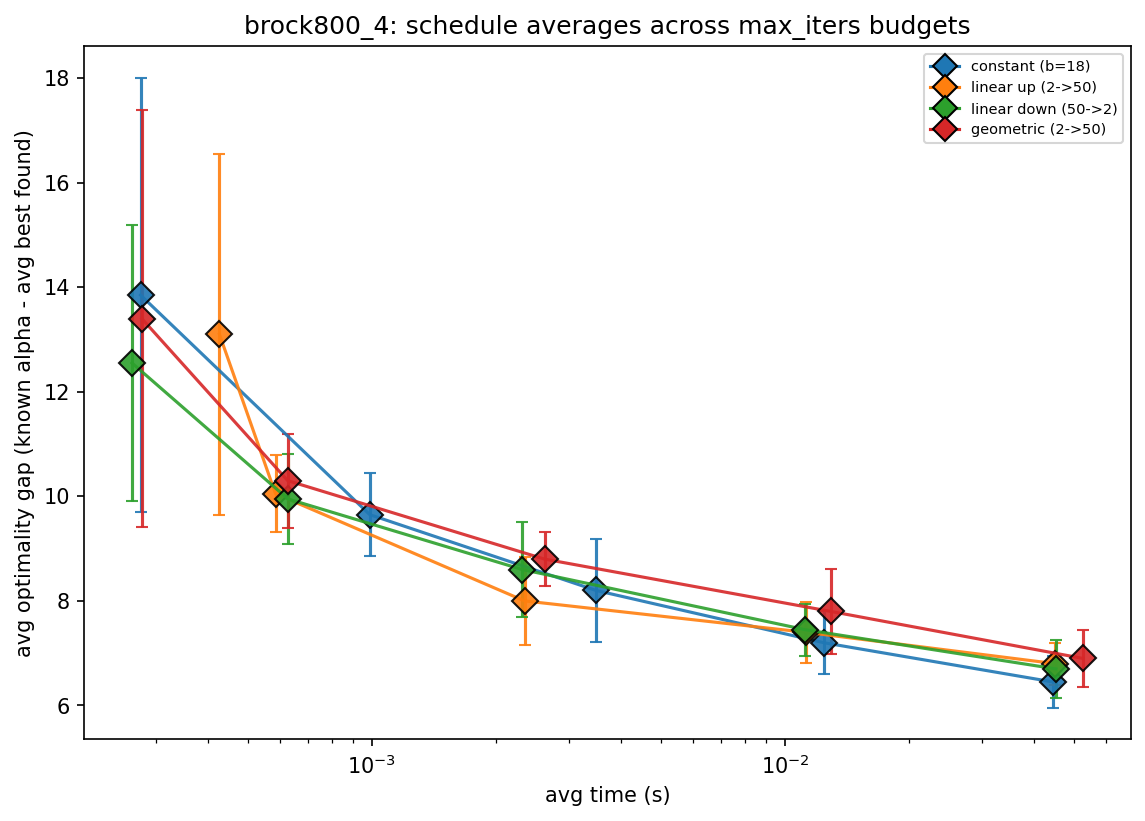
\includegraphics[width=0.5\textwidth]{../results/schedule_budget_sweep_brock800_4.png}
        \caption{Povprečno odstopanje od optimalne rešitve za različne strategije spreminjanja baze.}
        \label{fig:variable_base}
    \end{figure}
    \begin{figure}[H]
        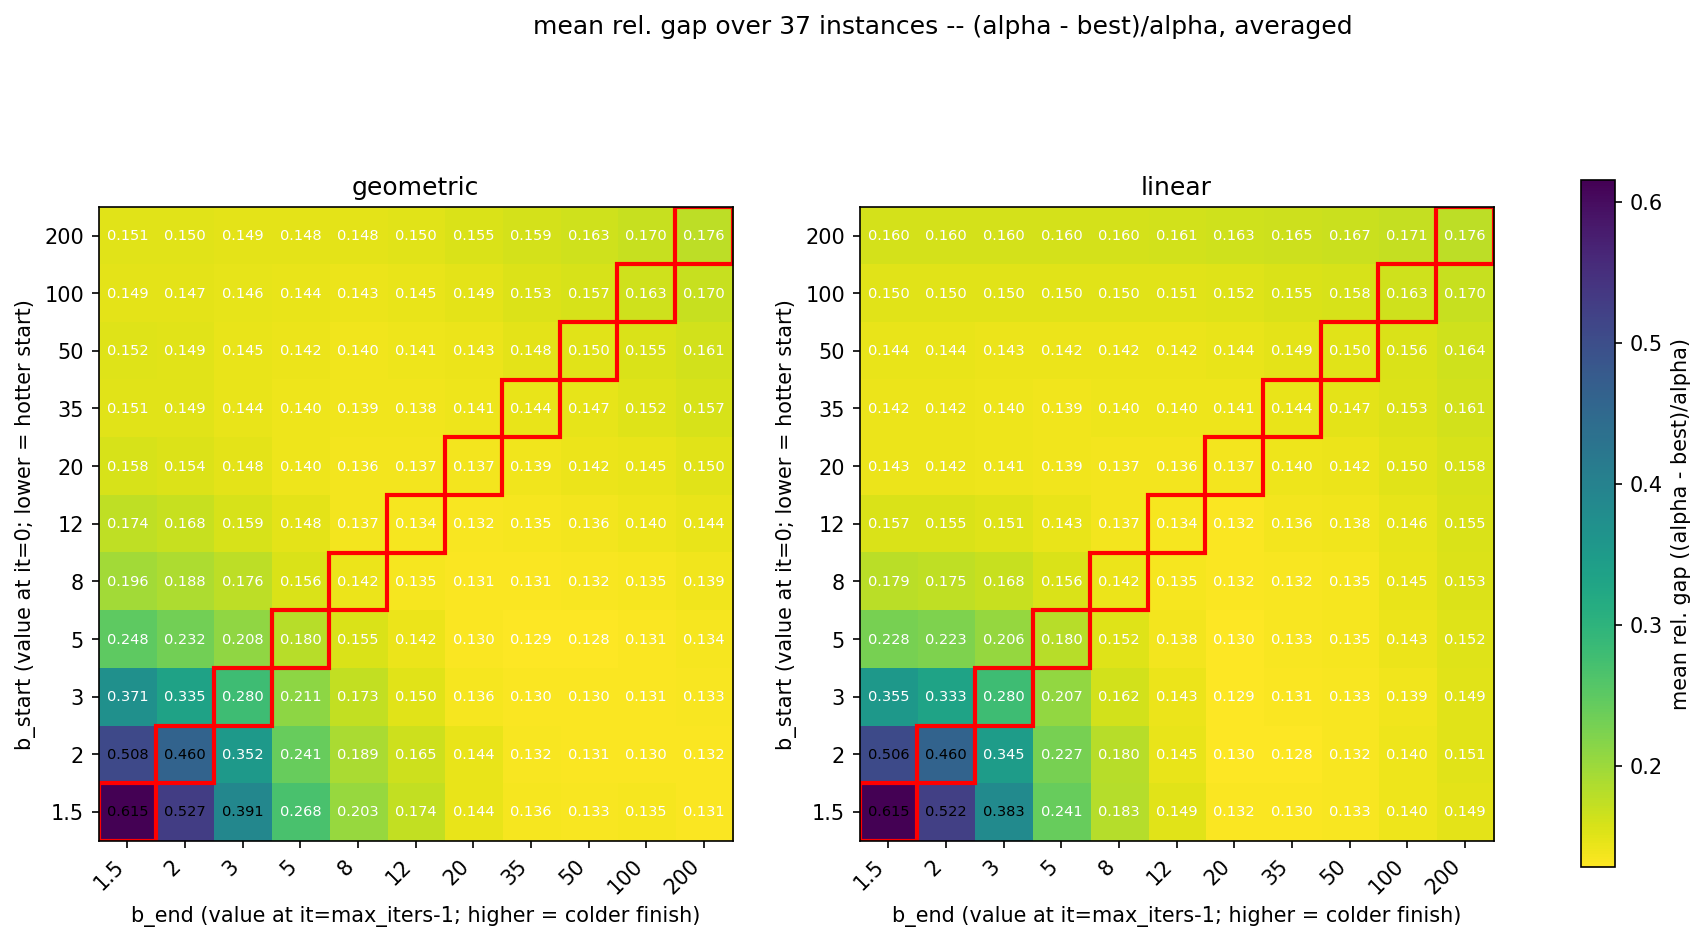
\includegraphics[width=\textwidth]{../results/schedule_sweep_all_instances_geometric-linear.png}
        \caption{Relativno odstopanje od optimalne rešitve v odvisnosti od začetne in končne vrednosti baze. Rdeči kvadrati označujejo fiksno bazo.}
        \label{fig:variable_base_all}
    \end{figure}

    \subsection{Spreminjanje razmerja $B/A$}
    Podobno stvar lahko ponovimo tudi za razmerje $B/A$.
    Ideja je, da bi začeli z večjim razmerjem $B/A$, da bi na začetku, ko imamo precej prazno množico, hitreje dodajali vozlišča, potem pa bi razmerje $B/A$ znižali, da bi prioritizirali stabilnost množice.
    Spodnja slika \ref{fig:variable_ratio} kaže relativno povprečno odstopanje od optimalne rešitve za različne strategije spreminjanja razmerja $B/A$.
    Razlike med tem in fiksnim razmerjem skoraj ni, najboljše vrednosti pa so dosežene pri razmerju $1.5 - 2$.

    \begin{figure}[H]
        \centering
        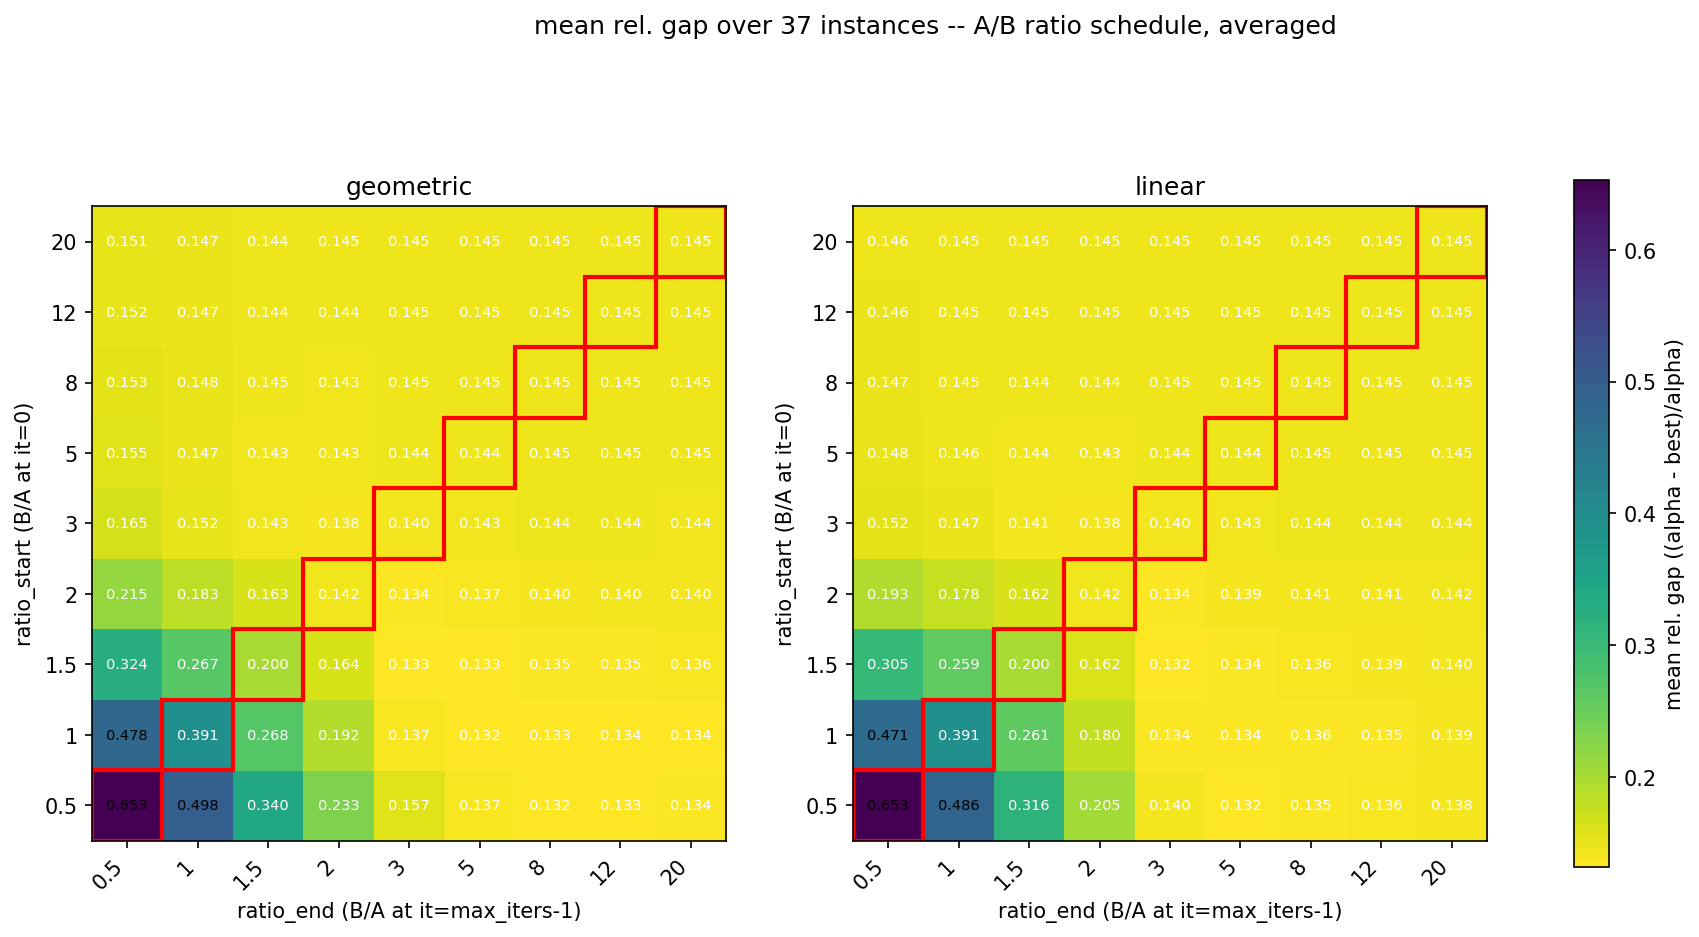
\includegraphics[width=\textwidth]{../results/ratio_schedule_sweep_all_instances_geometric-linear.png}
        \caption{Relativno odstopanje od optimalne rešitve v odvisnosti od začetne in končne vrednosti razmerja $B/A$. Rdeči kvadrati označujejo fiksno razmerje $B/A$.}
        \label{fig:variable_ratio}
    \end{figure}


    \section{Solver}
    \label{sec:solver}
    Očitno spreminjanje baze in razmerja $B/A$ tekom izvajanja ene ponovitve algoritma ne prinese boljših rezultatov, kot če bi uporabili fiksne vrednosti.
    Hkrati pa ne obstajajo optimalne vrednosti parametrov, ki bi bile dobre za vse primere.
    Zato sem se odločil, da namesto tega, da za vse ponovitve algoritma uporabim iste parametre, bom za vsako ponovitev izbral druge vrednosti.
    Za bazo sem uzel vrednosti $b \in \{1.5, 2.0, 3.0, 5.0, 8.0, 10.0, 15.0, 20.0, 30.0, 50.0\}$, za razmerje $B/A$ pa vrednosti $r \in \{1.0, 1.5, 2.0, 2.5, 3.0, 3.5, 4.0, 4.5, 5.0, 5.5\}$.
    Nato naredim kartezičnni produkt teh dveh množic in za vsako ponovitev po vrsti izberem en par parametrov. \\
    Namesto točne izbire števila iteracij, sem algoritem za vsako instanco izvajal po $1$ sekundo, kar je za vsako prišlo različno število iteracij.
    Tabela \ref{tab:results_solver} prikazuje rezultate izvajanja algoritma na vseh testnih instancah.
    \begin{longtable}{llrrrrrll}
\toprule
instance & upper\_bound & n & m & best & mean & elapsed\_sec & gap & relative\_gap \\
\midrule
\endfirsthead
\toprule
instance & upper\_bound & n & m & best & mean & elapsed\_sec & gap & relative\_gap \\
\midrule
\endhead
\midrule
\multicolumn{9}{r}{Continued on next page} \\
\midrule
\endfoot
\bottomrule
\endlastfoot
1dc.1024 & 94 & 1024 & 24063 & 73 & 32.53 & 0.11 & 21 & 0.2234 \\
1dc.128 & 16 & 128 & 1471 & 16 & 12.43 & 0.10 & 0 & 0.0000 \\
1dc.2048 & 174 & 2048 & 58367 & 122 & 24.36 & 0.12 & 52 & 0.2989 \\
1dc.256 & 30 & 256 & 3839 & 27 & 18.55 & 0.10 & 3 & 0.1000 \\
1dc.512 & 52 & 512 & 9727 & 42 & 28.54 & 0.10 & 10 & 0.1923 \\
1dc.64 & 10 & 64 & 543 & 10 & 8.39 & 0.11 & 0 & 0.0000 \\
1et.1024 & 171 & 1024 & 9600 & 155 & 50.75 & 0.11 & 16 & 0.0936 \\
1et.128 & 28 & 128 & 672 & 28 & 22.95 & 0.11 & 0 & 0.0000 \\
1et.2048 & 316 & 2048 & 22528 & 41 & 15.05 & 0.12 & 275 & 0.8703 \\
1et.256 & 50 & 256 & 1664 & 50 & 34.20 & 0.10 & 0 & 0.0000 \\
1et.512 & 100 & 512 & 4032 & 91 & 56.08 & 0.10 & 9 & 0.0900 \\
1et.64 & 18 & 64 & 264 & 18 & 16.32 & 0.11 & 0 & 0.0000 \\
1tc.1024 & 196 & 1024 & 7936 & 180 & 59.27 & 0.11 & 16 & 0.0816 \\
1tc.128 & 38 & 128 & 512 & 37 & 28.10 & 0.10 & 1 & 0.0263 \\
1tc.16 & 8 & 16 & 22 & 8 & 7.87 & 0.12 & 0 & 0.0000 \\
1tc.2048 & 352 & 2048 & 18944 & 42 & 16.60 & 0.12 & 310 & 0.8807 \\
1tc.256 & 63 & 256 & 1312 & 60 & 39.42 & 0.10 & 3 & 0.0476 \\
1tc.32 & 12 & 32 & 68 & 12 & 11.57 & 0.11 & 0 & 0.0000 \\
1tc.512 & 110 & 512 & 3264 & 105 & 60.87 & 0.10 & 5 & 0.0455 \\
1tc.64 & 20 & 64 & 192 & 20 & 17.73 & 0.11 & 0 & 0.0000 \\
1tc.8 & 4 & 8 & 6 & 4 & 4.00 & 0.15 & 0 & 0.0000 \\
1zc.1024 & 117 & 1024 & 16640 & 99 & 43.57 & 0.11 & 18 & 0.1538 \\
1zc.128 & 18 & 128 & 1120 & 18 & 14.49 & 0.11 & 0 & 0.0000 \\
1zc.2048 & 210 & 2048 & 39424 & 168 & 26.91 & 0.12 & 42 & 0.2000 \\
1zc.256 & 36 & 256 & 2816 & 36 & 23.45 & 0.10 & 0 & 0.0000 \\
1zc.4096 & 410 & 4096 & 92160 & 30 & 15.55 & 0.13 & 380 & 0.9268 \\
1zc.512 & 62 & 512 & 6912 & 61 & 36.84 & 0.10 & 1 & 0.0161 \\
2dc.1024 & 16 & 1024 & 169162 & 14 & 8.02 & 0.11 & 2 & 0.1250 \\
2dc.128 & 5 & 128 & 5173 & 5 & 4.53 & 0.11 & 0 & 0.0000 \\
2dc.2048 & 24 & 2048 & 504451 & 19 & 5.68 & 0.14 & 5 & 0.2083 \\
2dc.256 & 7 & 256 & 17183 & 7 & 5.56 & 0.10 & 0 & 0.0000 \\
2dc.512 & 11 & 512 & 54895 & 10 & 7.11 & 0.10 & 1 & 0.0909 \\
C125.9 & 34 & 125 & 787 & 34 & 27.09 & 0.10 & 0 & 0.0000 \\
MANN\_a9 & 16 & 45 & 72 & 16 & 14.93 & 0.11 & 0 & 0.0000 \\
a265032\_1dc.64-c &  & 64 & 1473 & 7 & 6.82 & 0.11 &  &  \\
a265032\_1et.128-c &  & 128 & 7456 & 7 & 5.87 & 0.11 &  &  \\
a265032\_1et.64-c &  & 64 & 1752 & 7 & 5.75 & 0.11 &  &  \\
a265032\_1tc.128-c &  & 128 & 7616 & 7 & 5.43 & 0.11 &  &  \\
a265032\_1tc.64-c &  & 64 & 1824 & 6 & 5.00 & 0.11 &  &  \\
a265032\_1zc.128-c &  & 128 & 7008 & 8 & 6.21 & 0.10 &  &  \\
a265032\_2dc.128-c &  & 128 & 2955 & 35 & 31.32 & 0.11 &  &  \\
brock200-4 & 17 & 200 & 6811 & 16 & 11.93 & 0.10 & 1 & 0.0588 \\
brock800\_1 & 23 & 800 & 112095 & 19 & 13.17 & 0.11 & 4 & 0.1739 \\
brock800\_2 & 24 & 800 & 111434 & 19 & 13.32 & 0.11 & 5 & 0.2083 \\
brock800\_3 & 25 & 800 & 112267 & 19 & 13.45 & 0.11 & 6 & 0.2400 \\
brock800\_4 & 26 & 800 & 111957 & 18 & 12.87 & 0.10 & 8 & 0.3077 \\
c-fat200-1 & 12 & 200 & 18366 & 12 & 10.65 & 0.10 & 0 & 0.0000 \\
c-fat200-2 & 24 & 200 & 16665 & 24 & 21.64 & 0.10 & 0 & 0.0000 \\
c-fat200-5 & 58 & 200 & 11427 & 58 & 54.28 & 0.10 & 0 & 0.0000 \\
c-fat500-1 & 14 & 500 & 120291 & 14 & 12.14 & 0.11 & 0 & 0.0000 \\
c-fat500-2 & 26 & 500 & 115611 & 26 & 24.24 & 0.11 & 0 & 0.0000 \\
c-fat500-5 & 64 & 500 & 101559 & 64 & 58.73 & 0.11 & 0 & 0.0000 \\
dsjc125.5 & 10 & 125 & 3859 & 10 & 7.94 & 0.10 & 0 & 0.0000 \\
dsjc125.9 & 34 & 125 & 789 & 34 & 26.80 & 0.10 & 0 & 0.0000 \\
evil-N100-p98-g136x10 &  & 100 & 4894 & 3 & 2.74 & 0.11 &  &  \\
evil-N100-p98-g150x10 &  & 100 & 4923 & 2 & 1.90 & 0.10 &  &  \\
evil-N100-p98-g50634x5 &  & 100 & 4843 & 3 & 2.13 & 0.10 &  &  \\
evil-N100-p98-myc5x20 &  & 100 & 4761 & 3 & 2.36 & 0.11 &  &  \\
evil-N100-p98-s3m25x4 &  & 100 & 4278 & 4 & 3.93 & 0.10 &  &  \\
evil-N108-p98-chv12x9 &  & 108 & 5286 & 4 & 3.89 & 0.10 &  &  \\
evil-N108-p98-g33896x6 &  & 108 & 5254 & 4 & 3.68 & 0.12 &  &  \\
evil-N108-p98-g33918x6 &  & 108 & 5319 & 4 & 3.69 & 0.10 &  &  \\
evil-N110-p98-g32559x10 &  & 110 & 5889 & 2 & 1.96 & 0.10 &  &  \\
evil-N110-p98-g32565x10 &  & 110 & 5804 & 3 & 2.24 & 0.11 &  &  \\
evil-N114-p98-g33920x6 &  & 114 & 5879 & 4 & 3.63 & 0.11 &  &  \\
evil-N115-p98-myc23x5 &  & 115 & 5540 & 11 & 10.19 & 0.10 &  &  \\
evil-N120-p98-chv12x10 & 20 & 120 & 545 & 20 & 16.67 & 0.10 & 0 & 0.0000 \\
evil-N120-p98-g136x12 &  & 120 & 7057 & 3 & 2.73 & 0.11 &  &  \\
evil-N120-p98-g50634x6 &  & 120 & 6991 & 3 & 2.08 & 0.11 &  &  \\
evil-N120-p98-myc5x24 & 48 & 120 & 236 & 48 & 37.57 & 0.10 & 0 & 0.0000 \\
evil-N121-p98-myc11x11 & 22 & 121 & 508 & 22 & 18.27 & 0.10 & 0 & 0.0000 \\
evil-N125-p98-s3m25x5 & 20 & 125 & 873 & 20 & 17.02 & 0.11 & 0 & 0.0000 \\
evil-N126-p98-g33896x7 &  & 126 & 7263 & 4 & 3.68 & 0.10 &  &  \\
evil-N126-p98-g33918x7 &  & 126 & 7322 & 4 & 3.69 & 0.10 &  &  \\
evil-N138-p98-myc23x6 &  & 138 & 8211 & 11 & 10.07 & 0.10 &  &  \\
evil-N150-p98-myc5x30 &  & 150 & 10837 & 3 & 2.51 & 0.11 &  &  \\
evil-N150-p98-s3m25x6 &  & 150 & 10073 & 4 & 3.87 & 0.10 &  &  \\
evil-N154-p98-myc11x14 &  & 154 & 11080 & 5 & 4.57 & 0.10 &  &  \\
evil-N180-p98-chv12x15 &  & 180 & 15166 & 4 & 3.83 & 0.11 &  &  \\
evil-N180-p98-myc5x36 &  & 180 & 15671 & 3 & 2.39 & 0.10 &  &  \\
evil-N184-p98-myc23x8 &  & 184 & 15072 & 11 & 10.08 & 0.10 &  &  \\
evil-N187-p98-myc11x17 &  & 187 & 16490 & 5 & 4.47 & 0.10 &  &  \\
evil-N200-p98-s3m25x8 &  & 200 & 18350 & 4 & 3.85 & 0.10 &  &  \\
evil-N210-p98-myc5x42 &  & 210 & 21404 & 3 & 2.50 & 0.11 &  &  \\
evil-N220-p98-myc11x20 &  & 220 & 22960 & 5 & 4.41 & 0.11 &  &  \\
evil-N230-p98-myc23x10 &  & 230 & 24072 & 11 & 10.01 & 0.10 &  &  \\
evil-N240-p98-chv12x20 &  & 240 & 27328 & 4 & 3.79 & 0.10 &  &  \\
evil-N240-p98-myc5x48 &  & 240 & 27962 & 3 & 2.47 & 0.11 &  &  \\
evil-N250-p98-s3m25x10 &  & 250 & 29075 & 4 & 3.81 & 0.10 &  &  \\
evil-N253-p98-myc11x23 &  & 253 & 30422 & 5 & 4.45 & 0.10 &  &  \\
evil-N300-p98-myc5x60 &  & 300 & 43817 & 4 & 2.57 & 0.10 &  &  \\
evil-N330-p98-myc11x30 &  & 330 & 52250 & 5 & 4.31 & 0.10 &  &  \\
evil-N345-p98-myc23x15 &  & 345 & 55473 & 11 & 9.69 & 0.10 &  &  \\
evil-N360-p98-chv12x30 &  & 360 & 62242 & 4 & 3.63 & 0.10 &  &  \\
evil-N375-p98-s3m25x15 &  & 375 & 66512 & 4 & 3.73 & 0.10 &  &  \\
evil-N400-p98-myc5x80 &  & 400 & 78138 & 3 & 2.40 & 0.10 &  &  \\
evil-N440-p98-myc11x40 &  & 440 & 93379 & 5 & 4.18 & 0.10 &  &  \\
evil-N460-p98-myc23x20 &  & 460 & 99906 & 11 & 9.75 & 0.11 &  &  \\
evil-N480-p98-chv12x40 &  & 480 & 111115 & 4 & 3.62 & 0.11 &  &  \\
evil-N50-p98-s3m25x2 &  & 50 & 910 & 4 & 3.97 & 0.11 &  &  \\
evil-N500-p98-myc5x100 &  & 500 & 122241 & 4 & 2.60 & 0.11 &  &  \\
evil-N500-p98-s3m25x20 &  & 500 & 119421 & 4 & 3.72 & 0.10 &  &  \\
evil-N55-p98-myc11x5 &  & 55 & 1288 & 5 & 4.75 & 0.11 &  &  \\
evil-N550-p98-myc11x50 &  & 550 & 146383 & 5 & 4.17 & 0.11 &  &  \\
evil-N575-p98-myc23x25 &  & 575 & 157386 & 11 & 9.37 & 0.11 &  &  \\
evil-N60-p98-chv12x5 &  & 60 & 1525 & 4 & 3.96 & 0.11 &  &  \\
evil-N60-p98-g136x6 &  & 60 & 1742 & 3 & 2.80 & 0.11 &  &  \\
evil-N60-p98-g150x6 &  & 60 & 1759 & 2 & 1.89 & 0.11 &  &  \\
evil-N60-p98-g50634x3 &  & 60 & 1720 & 2 & 1.98 & 0.12 &  &  \\
evil-N60-p98-myc5x12 &  & 60 & 1680 & 3 & 2.39 & 0.12 &  &  \\
evil-N600-p98-myc5x120 &  & 600 & 176037 & 3 & 2.61 & 0.11 &  &  \\
evil-N625-p98-s3m25x25 &  & 625 & 187602 & 4 & 3.61 & 0.11 &  &  \\
evil-N66-p98-g32559x6 &  & 66 & 2095 & 2 & 1.97 & 0.10 &  &  \\
evil-N66-p98-g32565x6 &  & 66 & 2059 & 3 & 2.22 & 0.11 &  &  \\
evil-N660-p98-myc11x60 &  & 660 & 211168 & 5 & 4.03 & 0.11 &  &  \\
evil-N69-p98-myc23x3 &  & 69 & 1759 & 11 & 10.29 & 0.10 &  &  \\
evil-N690-p98-myc23x30 &  & 690 & 227627 & 11 & 9.41 & 0.11 &  &  \\
evil-N700-p98-myc5x140 &  & 700 & 239865 & 4 & 2.58 & 0.12 &  &  \\
evil-N72-p98-chv12x6 &  & 72 & 2250 & 4 & 3.92 & 0.11 &  &  \\
evil-N72-p98-g33896x4 &  & 72 & 2237 & 4 & 3.72 & 0.11 &  &  \\
evil-N72-p98-g33918x4 &  & 72 & 2273 & 4 & 3.72 & 0.12 &  &  \\
evil-N720-p98-chv12x60 &  & 720 & 251425 & 4 & 3.48 & 0.12 &  &  \\
evil-N75-p98-s3m25x3 &  & 75 & 2292 & 4 & 3.96 & 0.11 &  &  \\
evil-N750-p98-s3m25x30 &  & 750 & 271062 & 5 & 3.48 & 0.12 &  &  \\
evil-N76-p98-g33920x4 &  & 76 & 2501 & 4 & 3.64 & 0.12 &  &  \\
evil-N77-p98-myc11x7 &  & 77 & 2626 & 5 & 4.66 & 0.10 &  &  \\
evil-N80-p98-g136x8 &  & 80 & 3116 & 3 & 2.79 & 0.11 &  &  \\
evil-N80-p98-g150x8 &  & 80 & 3139 & 2 & 1.90 & 0.10 &  &  \\
evil-N80-p98-g50634x4 &  & 80 & 3079 & 3 & 2.18 & 0.10 &  &  \\
evil-N80-p98-myc5x16 &  & 80 & 3036 & 3 & 2.42 & 0.11 &  &  \\
evil-N84-p98-chv12x7 &  & 84 & 3126 & 4 & 3.92 & 0.10 &  &  \\
evil-N88-p98-g32559x8 &  & 88 & 3733 & 3 & 2.19 & 0.10 &  &  \\
evil-N88-p98-g32565x8 &  & 88 & 3695 & 3 & 2.14 & 0.10 &  &  \\
evil-N90-p98-g33896x5 &  & 90 & 3585 & 4 & 3.69 & 0.10 &  &  \\
evil-N90-p98-g33918x5 &  & 90 & 3637 & 4 & 3.74 & 0.10 &  &  \\
evil-N92-p98-myc23x4 &  & 92 & 3404 & 11 & 10.26 & 0.11 &  &  \\
evil-N95-p98-g33920x5 &  & 95 & 4031 & 4 & 3.63 & 0.10 &  &  \\
evil-N96-p98-chv12x8 &  & 96 & 4152 & 4 & 3.91 & 0.11 &  &  \\
evil-N99-p98-myc11x9 &  & 99 & 4445 & 5 & 4.63 & 0.11 &  &  \\
frb100-40 &  & 4000 & 572774 & 12 & 6.73 & 0.14 &  &  \\
frb30-15-1 & 30 & 450 & 17827 & 26 & 19.12 & 0.10 & 4 & 0.1333 \\
frb30-15-2 & 30 & 450 & 17874 & 27 & 19.46 & 0.10 & 3 & 0.1000 \\
frb30-15-3 & 30 & 450 & 17809 & 27 & 18.98 & 0.10 & 3 & 0.1000 \\
frb30-15-4 & 30 & 450 & 17831 & 28 & 19.10 & 0.10 & 2 & 0.0667 \\
frb30-15-5 & 30 & 450 & 17794 & 27 & 19.28 & 0.10 & 3 & 0.1000 \\
frb35-17-1 & 35 & 595 & 27856 & 32 & 20.75 & 0.10 & 3 & 0.0857 \\
frb35-17-2 & 35 & 595 & 27847 & 31 & 21.14 & 0.10 & 4 & 0.1143 \\
frb35-17-3 & 35 & 595 & 27931 & 31 & 21.05 & 0.10 & 4 & 0.1143 \\
frb35-17-4 & 35 & 595 & 27842 & 30 & 21.37 & 0.10 & 5 & 0.1429 \\
frb35-17-5 & 35 & 595 & 28143 & 30 & 20.28 & 0.10 & 5 & 0.1429 \\
frb40-19-1 & 40 & 760 & 41314 & 34 & 20.70 & 0.10 & 6 & 0.1500 \\
frb40-19-2 & 40 & 760 & 41263 & 35 & 21.63 & 0.10 & 5 & 0.1250 \\
frb40-19-3 & 40 & 760 & 41095 & 35 & 20.87 & 0.10 & 5 & 0.1250 \\
frb40-19-4 & 40 & 760 & 41605 & 34 & 21.56 & 0.11 & 6 & 0.1500 \\
frb40-19-5 & 40 & 760 & 41619 & 35 & 21.44 & 0.10 & 5 & 0.1250 \\
frb45-21-1 & 45 & 945 & 59186 & 40 & 21.75 & 0.11 & 5 & 0.1111 \\
frb45-21-2 & 45 & 945 & 58624 & 38 & 20.73 & 0.11 & 7 & 0.1556 \\
frb45-21-3 & 45 & 945 & 58245 & 38 & 20.76 & 0.11 & 7 & 0.1556 \\
frb45-21-4 & 45 & 945 & 58549 & 38 & 20.55 & 0.11 & 7 & 0.1556 \\
frb45-21-5 & 45 & 945 & 58579 & 38 & 21.47 & 0.11 & 7 & 0.1556 \\
frb50-23-1 & 50 & 1150 & 80072 & 43 & 20.29 & 0.11 & 7 & 0.1400 \\
frb50-23-2 & 50 & 1150 & 80851 & 43 & 21.22 & 0.12 & 7 & 0.1400 \\
frb50-23-3 & 50 & 1150 & 81068 & 42 & 21.76 & 0.11 & 8 & 0.1600 \\
frb50-23-4 & 50 & 1150 & 80258 & 43 & 20.88 & 0.11 & 7 & 0.1400 \\
frb50-23-5 & 50 & 1150 & 80035 & 42 & 21.20 & 0.11 & 8 & 0.1600 \\
frb53-24-1 & 53 & 1272 & 94227 & 44 & 19.27 & 0.11 & 9 & 0.1698 \\
frb53-24-2 & 53 & 1272 & 94289 & 47 & 20.76 & 0.11 & 6 & 0.1132 \\
frb53-24-3 & 53 & 1272 & 94127 & 44 & 19.89 & 0.11 & 9 & 0.1698 \\
frb53-24-4 & 53 & 1272 & 94308 & 44 & 20.59 & 0.11 & 9 & 0.1698 \\
frb53-24-5 & 53 & 1272 & 94226 & 45 & 20.54 & 0.11 & 8 & 0.1509 \\
frb59-26-1 & 59 & 1534 & 126555 & 50 & 20.13 & 0.11 & 9 & 0.1525 \\
frb59-26-2 & 59 & 1534 & 126163 & 50 & 19.77 & 0.11 & 9 & 0.1525 \\
frb59-26-3 & 59 & 1534 & 126082 & 50 & 19.87 & 0.11 & 9 & 0.1525 \\
frb59-26-4 & 59 & 1534 & 127011 & 50 & 21.43 & 0.11 & 9 & 0.1525 \\
frb59-26-5 & 59 & 1534 & 125982 & 49 & 19.87 & 0.12 & 10 & 0.1695 \\
hamming6-2 &  & 64 & 1824 & 2 & 1.98 & 0.11 &  &  \\
hamming6-4 &  & 64 & 704 & 12 & 11.52 & 0.11 &  &  \\
hamming6\_2 & 32 & 64 & 192 & 32 & 29.07 & 0.11 & 0 & 0.0000 \\
hamming6\_4 & 4 & 64 & 1312 & 4 & 3.91 & 0.11 & 0 & 0.0000 \\
johnson16-2-4 &  & 120 & 5460 & 15 & 14.63 & 0.10 &  &  \\
johnson16\_2\_4 & 8 & 120 & 1680 & 8 & 7.35 & 0.10 & 0 & 0.0000 \\
johnson8-4-4 &  & 70 & 1855 & 5 & 4.92 & 0.10 &  &  \\
johnson8\_2\_4 & 4 & 28 & 168 & 4 & 3.98 & 0.12 & 0 & 0.0000 \\
johnson8\_4\_4 & 14 & 70 & 560 & 14 & 12.37 & 0.11 & 0 & 0.0000 \\
keller4 & 11 & 171 & 5100 & 11 & 8.56 & 0.10 & 0 & 0.0000 \\
p-hat500-1 & 9 & 500 & 93181 & 9 & 6.97 & 0.10 & 0 & 0.0000 \\
p\_hat1500\_1 & 12 & 1500 & 839327 & 11 & 6.83 & 0.15 & 1 & 0.0833 \\
p\_hat1500\_2 & 65 & 1500 & 555290 & 64 & 27.24 & 0.13 & 1 & 0.0154 \\
p\_hat1500\_3 & 94 & 1500 & 277006 & 89 & 33.44 & 0.12 & 5 & 0.0532 \\
paley101 &  & 101 & 2525 & 5 & 4.85 & 0.10 &  &  \\
paley61 &  & 61 & 915 & 5 & 4.92 & 0.11 &  &  \\
paley73 &  & 73 & 1314 & 5 & 4.86 & 0.10 &  &  \\
paley89 &  & 89 & 1958 & 5 & 4.85 & 0.10 &  &  \\
paley97 &  & 97 & 2328 & 6 & 5.84 & 0.10 &  &  \\
san200-0-7-1 & 30 & 200 & 5970 & 30 & 12.22 & 0.10 & 0 & 0.0000 \\
san200-0-7-2 & 18 & 200 & 5970 & 15 & 9.74 & 0.10 & 3 & 0.1667 \\
sanr200-0-7 & 18 & 200 & 6032 & 18 & 13.44 & 0.10 & 0 & 0.0000 \\
vc-exact\_001 & 3574 & 6160 & 40207 & 81 & 39.00 & 0.12 & 3493 & 0.9773 \\
vc-exact\_003 & 48351 & 60541 & 48418 & 211 & 211.00 & 0.28 & 48140 & 0.9956 \\
vc-exact\_005 & 71 & 200 & 798 & 71 & 51.01 & 0.10 & 0 & 0.0000 \\
vc-exact\_007 & 4397 & 8794 & 10121 & 186 & 80.67 & 0.14 & 4211 & 0.9577 \\
vc-exact\_009 & 17104 & 38452 & 174645 & 129 & 129.00 & 0.20 & 16975 & 0.9925 \\
vc-exact\_011 & 4896 & 9877 & 25973 & 77 & 49.00 & 0.11 & 4819 & 0.9843 \\
vc-exact\_013 & 36697 & 45307 & 36697 & 144 & 144.00 & 0.21 & 36553 & 0.9961 \\
vc-exact\_015 & 42940 & 53610 & 42940 & 476 & 476.00 & 0.25 & 42464 & 0.9889 \\
vc-exact\_017 & 11459 & 23541 & 34233 & 25 & 25.00 & 0.13 & 11434 & 0.9978 \\
vc-exact\_019 & 70 & 200 & 862 & 69 & 50.53 & 0.10 & 1 & 0.0143 \\
vc-exact\_021 & 19655 & 24765 & 19655 & 529 & 529.00 & 0.12 & 19126 & 0.9731 \\
vc-exact\_023 & 11704 & 27717 & 133665 & 27 & 27.00 & 0.16 & 11677 & 0.9977 \\
vc-exact\_025 & 18295 & 23194 & 18295 & 549 & 549.00 & 0.13 & 17746 & 0.9700 \\
vc-exact\_027 & 52435 & 65866 & 52435 & 857 & 857.00 & 0.30 & 51578 & 0.9837 \\
vc-exact\_029 & 6809 & 13431 & 16234 & 67 & 67.00 & 0.08 & 6742 & 0.9902 \\
vc-exact\_031 & 64 & 200 & 813 & 63 & 43.58 & 0.12 & 1 & 0.0156 \\
vc-exact\_033 & 1685 & 4410 & 6885 & 105 & 54.67 & 0.13 & 1580 & 0.9377 \\
vc-exact\_035 & 67 & 200 & 864 & 65 & 46.43 & 0.10 & 2 & 0.0299 \\
vc-exact\_037 & 67 & 198 & 808 & 67 & 46.62 & 0.11 & 0 & 0.0000 \\
vc-exact\_039 & 2595 & 6795 & 10620 & 95 & 59.00 & 0.14 & 2500 & 0.9634 \\
vc-exact\_041 & 61 & 200 & 1023 & 59 & 43.32 & 0.10 & 2 & 0.0328 \\
vc-exact\_043 & 61 & 200 & 841 & 58 & 41.63 & 0.10 & 3 & 0.0492 \\
vc-exact\_045 & 63 & 200 & 1020 & 62 & 45.74 & 0.10 & 1 & 0.0159 \\
vc-exact\_047 & 60 & 200 & 1093 & 58 & 43.38 & 0.10 & 2 & 0.0333 \\
vc-exact\_049 & 64 & 200 & 933 & 62 & 45.29 & 0.10 & 2 & 0.0312 \\
vc-exact\_051 & 60 & 200 & 1098 & 60 & 42.34 & 0.12 & 0 & 0.0000 \\
vc-exact\_053 & 61 & 200 & 1026 & 60 & 43.04 & 0.10 & 1 & 0.0164 \\
vc-exact\_055 & 66 & 200 & 938 & 65 & 47.35 & 0.10 & 1 & 0.0152 \\
vc-exact\_057 & 58 & 200 & 1160 & 58 & 41.52 & 0.10 & 0 & 0.0000 \\
vc-exact\_059 & 63 & 200 & 961 & 62 & 45.29 & 0.10 & 1 & 0.0159 \\
vc-exact\_061 & 65 & 200 & 931 & 64 & 46.72 & 0.10 & 1 & 0.0154 \\
vc-exact\_063 & 62 & 200 & 1011 & 60 & 42.92 & 0.10 & 2 & 0.0323 \\
vc-exact\_065 & 62 & 200 & 1011 & 61 & 44.44 & 0.10 & 1 & 0.0161 \\
vc-exact\_067 & 57 & 200 & 1174 & 57 & 41.99 & 0.10 & 0 & 0.0000 \\
vc-exact\_069 & 60 & 200 & 1083 & 59 & 43.69 & 0.10 & 1 & 0.0167 \\
vc-exact\_071 & 64 & 200 & 952 & 62 & 45.68 & 0.10 & 2 & 0.0312 \\
vc-exact\_073 & 61 & 200 & 1078 & 59 & 43.64 & 0.10 & 2 & 0.0328 \\
vc-exact\_075 & 10000 & 26300 & 41500 & 244 & 244.00 & 0.15 & 9756 & 0.9756 \\
vc-exact\_079 & 10000 & 26300 & 41500 & 226 & 226.00 & 0.15 & 9774 & 0.9774 \\
vc-exact\_081 & 58 & 199 & 1091 & 56 & 42.26 & 0.10 & 2 & 0.0345 \\
vc-exact\_083 & 56 & 200 & 1172 & 55 & 40.21 & 0.10 & 1 & 0.0179 \\
vc-exact\_085 & 4436 & 11470 & 17408 & 116 & 99.00 & 0.13 & 4320 & 0.9739 \\
vc-exact\_087 & 5190 & 13590 & 21240 & 117 & 117.00 & 0.08 & 5073 & 0.9775 \\
vc-exact\_089 & 23178 & 57316 & 77978 & 135 & 135.00 & 0.32 & 23043 & 0.9942 \\
vc-exact\_091 & 55 & 200 & 1163 & 54 & 39.47 & 0.10 & 1 & 0.0182 \\
vc-exact\_093 & 57 & 200 & 1162 & 55 & 40.97 & 0.10 & 2 & 0.0351 \\
vc-exact\_095 & 6028 & 15783 & 24663 & 64 & 64.00 & 0.09 & 5964 & 0.9894 \\
vc-exact\_097 & 6911 & 18096 & 28281 & 80 & 80.00 & 0.10 & 6831 & 0.9884 \\
vc-exact\_099 & 10000 & 26300 & 41500 & 67 & 67.00 & 0.15 & 9933 & 0.9933 \\
vc-exact\_101 & 10000 & 26300 & 41500 & 244 & 244.00 & 0.15 & 9756 & 0.9756 \\
vc-exact\_103 & 6028 & 15783 & 24663 & 64 & 64.00 & 0.09 & 5964 & 0.9894 \\
vc-exact\_105 & 10000 & 26300 & 41500 & 116 & 116.00 & 0.15 & 9884 & 0.9884 \\
vc-exact\_107 & 5190 & 13590 & 21240 & 134 & 125.50 & 0.15 & 5056 & 0.9742 \\
vc-exact\_109 & 27110 & 66992 & 90970 & 125 & 125.00 & 0.37 & 26985 & 0.9954 \\
vc-exact\_113 & 10000 & 26300 & 41500 & 244 & 244.00 & 0.15 & 9756 & 0.9756 \\
vc-exact\_115 & 6911 & 18096 & 28281 & 80 & 80.00 & 0.10 & 6831 & 0.9884 \\
vc-exact\_117 & 6911 & 18096 & 28281 & 80 & 80.00 & 0.10 & 6831 & 0.9884 \\
vc-exact\_119 & 6911 & 18096 & 28281 & 80 & 80.00 & 0.10 & 6831 & 0.9884 \\
vc-exact\_121 & 6911 & 18096 & 28281 & 80 & 80.00 & 0.10 & 6831 & 0.9884 \\
vc-exact\_123 & 10000 & 26300 & 41500 & 244 & 244.00 & 0.15 & 9756 & 0.9756 \\
vc-exact\_125 & 10000 & 26300 & 41500 & 67 & 67.00 & 0.15 & 9933 & 0.9933 \\
vc-exact\_127 & 6911 & 18096 & 28281 & 66 & 66.00 & 0.10 & 6845 & 0.9905 \\
vc-exact\_129 & 6028 & 15783 & 24663 & 64 & 64.00 & 0.09 & 5964 & 0.9894 \\
vc-exact\_131 & 1060 & 2980 & 5360 & 73 & 36.00 & 0.13 & 987 & 0.9311 \\
vc-exact\_133 & 6028 & 15783 & 24663 & 64 & 64.00 & 0.09 & 5964 & 0.9894 \\
vc-exact\_135 & 10000 & 26300 & 41500 & 244 & 244.00 & 0.15 & 9756 & 0.9756 \\
vc-exact\_137 & 10000 & 26300 & 41500 & 243 & 243.00 & 0.14 & 9757 & 0.9757 \\
vc-exact\_139 & 6911 & 18096 & 28281 & 80 & 80.00 & 0.10 & 6831 & 0.9884 \\
vc-exact\_141 & 6911 & 18096 & 28281 & 80 & 80.00 & 0.10 & 6831 & 0.9884 \\
vc-exact\_143 & 6911 & 18096 & 28281 & 80 & 80.00 & 0.10 & 6831 & 0.9884 \\
vc-exact\_145 & 6911 & 18096 & 28281 & 80 & 80.00 & 0.10 & 6831 & 0.9884 \\
vc-exact\_147 & 6911 & 18096 & 28281 & 80 & 80.00 & 0.10 & 6831 & 0.9884 \\
vc-exact\_149 & 10000 & 26300 & 41500 & 244 & 244.00 & 0.15 & 9756 & 0.9756 \\
vc-exact\_151 & 6028 & 15783 & 24663 & 63 & 63.00 & 0.09 & 5965 & 0.9895 \\
vc-exact\_153 & 11083 & 29076 & 45570 & 170 & 170.00 & 0.16 & 10913 & 0.9847 \\
vc-exact\_155 & 10000 & 26300 & 41500 & 244 & 244.00 & 0.15 & 9756 & 0.9756 \\
vc-exact\_157 & 1060 & 2980 & 5360 & 90 & 48.80 & 0.13 & 970 & 0.9151 \\
vc-exact\_159 & 6911 & 18096 & 28281 & 80 & 80.00 & 0.10 & 6831 & 0.9884 \\
vc-exact\_161 & 51496 & 138141 & 227241 & 216 & 216.00 & 0.78 & 51280 & 0.9958 \\
vc-exact\_163 & 6911 & 18096 & 28281 & 80 & 80.00 & 0.11 & 6831 & 0.9884 \\
vc-exact\_165 & 6911 & 18096 & 28281 & 80 & 80.00 & 0.10 & 6831 & 0.9884 \\
vc-exact\_167 & 6028 & 15783 & 24663 & 64 & 64.00 & 0.09 & 5964 & 0.9894 \\
vc-exact\_169 & 1696 & 4768 & 8576 & 98 & 61.67 & 0.14 & 1598 & 0.9422 \\
vc-exact\_171 & 6911 & 18096 & 28281 & 80 & 80.00 & 0.10 & 6831 & 0.9884 \\
vc-exact\_173 & 23004 & 56860 & 77264 & 224 & 224.00 & 0.32 & 22780 & 0.9903 \\
vc-exact\_175 & 1241 & 3523 & 6446 & 123 & 63.00 & 0.14 & 1118 & 0.9009 \\
vc-exact\_177 & 1802 & 5066 & 9112 & 154 & 76.83 & 0.15 & 1648 & 0.9145 \\
vc-exact\_179 & 6028 & 15783 & 24663 & 64 & 64.00 & 0.09 & 5964 & 0.9894 \\
vc-exact\_181 & 6911 & 18096 & 28281 & 80 & 80.00 & 0.10 & 6831 & 0.9884 \\
vc-exact\_183 & 27082 & 72420 & 118362 & 350 & 350.00 & 0.41 & 26732 & 0.9871 \\
vc-exact\_185 & 1241 & 3523 & 6446 & 78 & 54.67 & 0.15 & 1163 & 0.9371 \\
vc-exact\_187 & 1489 & 4227 & 7734 & 80 & 54.71 & 0.14 & 1409 & 0.9463 \\
vc-exact\_189 & 2600 & 7400 & 13600 & 131 & 61.50 & 0.15 & 2469 & 0.9496 \\
vc-exact\_191 & 1613 & 4579 & 8378 & 121 & 82.33 & 0.13 & 1492 & 0.9250 \\
vc-exact\_193 & 2470 & 7030 & 12920 & 112 & 60.50 & 0.14 & 2358 & 0.9547 \\
\end{longtable}


    \section{Zaključek}
    Algoritem je precej hiter in da dobre rezultate.
    Zaenkrat večina predlaganih izboljšav ni prineslo boljših rezultatov, ampak bi se dalo še marsikaj poskusiti.
    V prihodnje bi lahko izboljšali algoritem za začetno stanje, da bi morda izboljšali rezultate, prav tako bi lahko dodali še kakšen postprocesing.
    Lahko bi tudi poskusil dodati boljšo oceno optimalne rešitve, kot le velikost trenutne množice minus število povezav v njej.
    Zaenkrat sem ločeno preizkušal spreminjanje baze in razmerja $B/A$, v prihodnje pa bi lahko poskusil tudi kombinirati oba postopka in videti, če bi to prineslo boljše rezultate.
    Razlika med tem in originalnim PW algoritmom je, da originalni ne izbere naključnega vozlišča, ampak izbere naključno slabo vozlišče.
    Morda bi lahko začeli z polno množico in na ta način odstranjevali vozlišča, dokler ne pridemo do stabilne rešitve.
    Prav tako bi lahko namesto naključnega izbora vozlišča, izbrali vozlišča po vrsti in tako zagotovili, da algoritem preišče cel graf enakomerno.

    \bibliography{refs}


\end{document}